\pagebreak
\subsection{Task 2: Build and Configure the Server Array}

\subsubsection{Download Windows Server 2016 ISO}
\begin{enumerate}[series=task2methodology1]
  \item Download Windows Server 2016 from the `Microsoft Imagine'\footnote{\url{https://imagine.microsoft.com/en-us}} website, as shown in Figure~\ref{fig:task2:winserver2016_download} in the \nameref{app:ancillaryscreenshots} appendix.
\end{enumerate}

\noindent I have taken a different approach for the next step to the normal approach of uploading the ISO via the vSphere Web Client or vSphere Client (desktop). This is due to a bug with ESXi 6.0.0 that prevents uploads when using the IPv6 address to access the instance's Web Client interface. When you use the `Datastore Browser' to upload a file, the upload freezes at 0\% and does not progress at all.

\subsubsection{Transfer the ISO into the ESXi instance}
\begin{enumerate}[resume*=task2methodology1]
  \item Use the Web Client to enable SSH access to the ESXi instance by going to `Host > Actions > Services > Enable Secure Shell (SSH)'.
  \item Download \texttt{pscp.exe} from the PuTTY website\footnote{\url{https://www.chiark.greenend.org.uk/~sgtatham/putty/latest.html}}.
  \item In the Web Client, find the path to `datastore1' by going to `Storage > datastore1' and viewing the `Location`. In my case, this was:\\ \texttt{/vmfs/volumes/5af1d3e9-abd56f67-0cdf-000c296b7530/}.
  \item On the workstation host where the ISO was downloaded, in PowerShell from the directory that the ISO resides in run:\\
  \texttt{C:\textbackslash tools\textbackslash pscp.exe -6}\\
  \texttt{.\textbackslash 14393.0.161119-1705.RS1\_REFRESH\_SERVER\_EVAL\_X64FRE\_EN-US.ISO}\\
  \texttt{root@[fe80::20c:29ff:fe6b:7530]:}\\
  \texttt{/vmfs/volumes/5af1d3e9-abd56f67-0cdf-000c296b7530/isos}\\
  This will secure copy the ISO to the ESXi instance over SSH.
\end{enumerate}

\noindent When not using the SSH service for remote administration, it should be disabled to reduce the attack surface of the ESXi instance. It should be noted that restarting the ESXi instance will automatically re-disable the SSH service.

\subsubsection{Install Windows Server 2016 in a new VM}
\begin{enumerate}[series=task2methodology2]
  \item Create a new VM in the Web Client for the ESXi instance. Notable steps are detailed forthwith:
    \begin{enumerate}[label=(\alph*)]
      \item Select `Create a new virtual machine` in the `Select creation type` step.
        \begin{figure}[H]
          \centering
          \captionsetup{skip=2pt}
          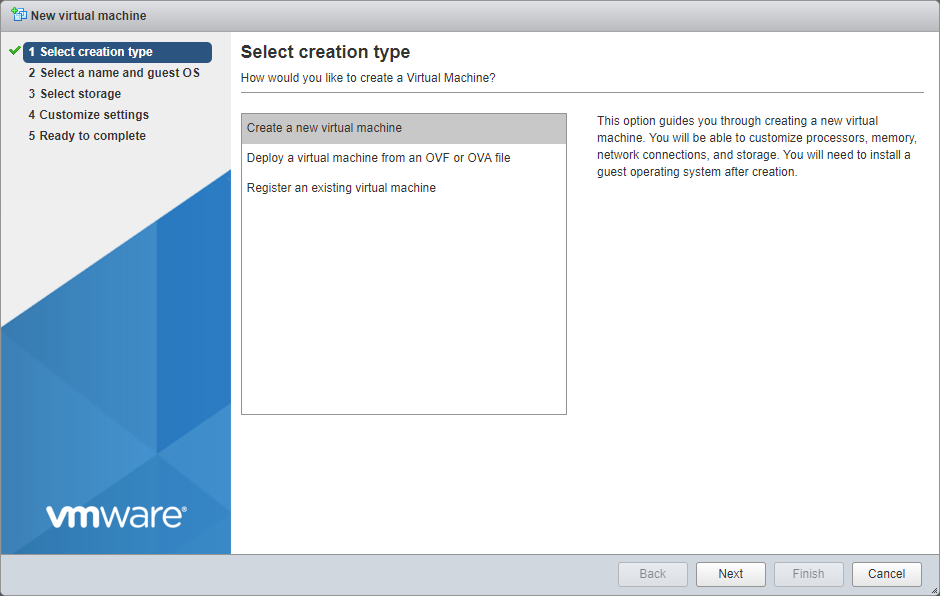
\includegraphics[width=\textwidth]{task2_06_winserver2016_2_dc_crop}
          \caption{Creating a new VM in ESXi}
          \label{fig:task2:vspherewc_newvm1}
        \end{figure}
      \item Give the VM a unique (within the ESXi instance) name and set the Guest OS Family and Version to be `Windows` and `Microsoft Windows Server 2016 (64-bit)` respectively.
        \begin{figure}[H]
          \centering
          \captionsetup{skip=2pt}
          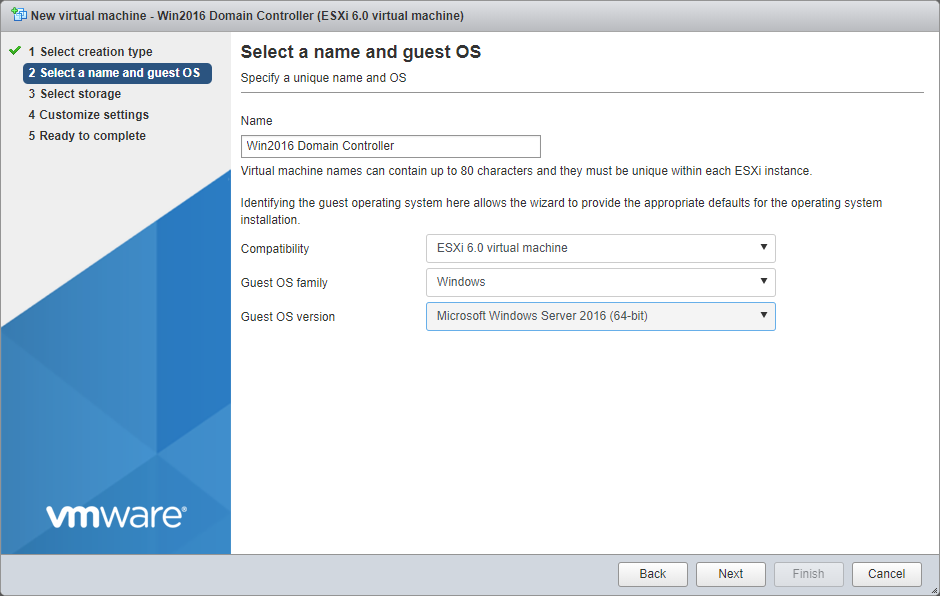
\includegraphics[width=\textwidth]{task2_06_winserver2016_3_dc_crop}
          \caption{Selecting the name and guest OS in the `New virtual machine` wizard}
          \label{fig:task2:vspherewc_newvm2}
        \end{figure}
      \item Mount the Windows Server 2016 ISO in the CD drive for the new virtual machine.
        \begin{figure}[H]
          \centering
          \captionsetup{skip=2pt}
          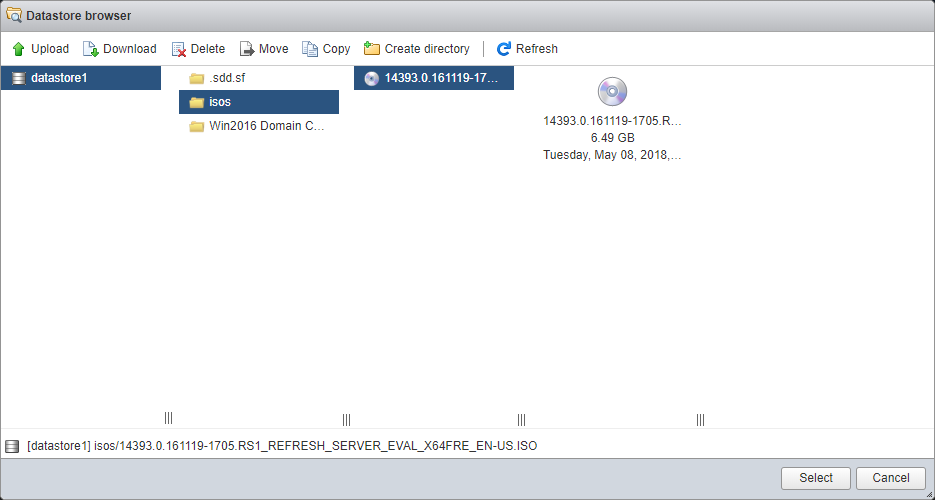
\includegraphics[width=\textwidth]{task2_06_winserver2016_9_dc_crop}
          \caption{Selecting the ISO to run at boot in the new VM}
          \label{fig:task2:vspherewc_newvm3}
        \end{figure}
    \end{enumerate}
\end{enumerate}

\noindent The screenshot in Figure~\ref{fig:task2:vspherewc_newvm4} in the \nameref{app:ancillaryscreenshots} appendix shows the Web Client UI display for the newly created VM.\\\\
\noindent For the next steps, I used the vSphere Client to display the console of specific VMs inside ESXi. This is primarily because of a bug in ESXi 6.0 that prevents consoles from being shown in the browser, as shown in Figures~\ref{fig:task2:vspherewc_bug1} and~\ref{fig:task2:vspherewc_bug2} in the \nameref{app:ancillaryscreenshots} appendix. However, the vSphere Client is also nicer to use as it responds faster and does not attempt to scale the console to the size of the browser window.

\begin{enumerate}[resume*=task2methodology2]
  \item \label{task2:installwin2016server} Open a console in the vSphere Client (desktop) to the newly created VM for Windows and start it.
  \item Install Windows Server in the VM. Notable steps include:
    \begin{enumerate}[label=(\alph*)]
      \item Choosing `Windows Server 2016 Datacenter Evaluation (Desktop Experience)' edition as shown in the image below. This is done to ensure that the full feature set required for the project is included in the installation and that a desktop is available to make the server easier to configure.
        \begin{figure}[H]
          \centering
          \captionsetup{skip=2pt}
          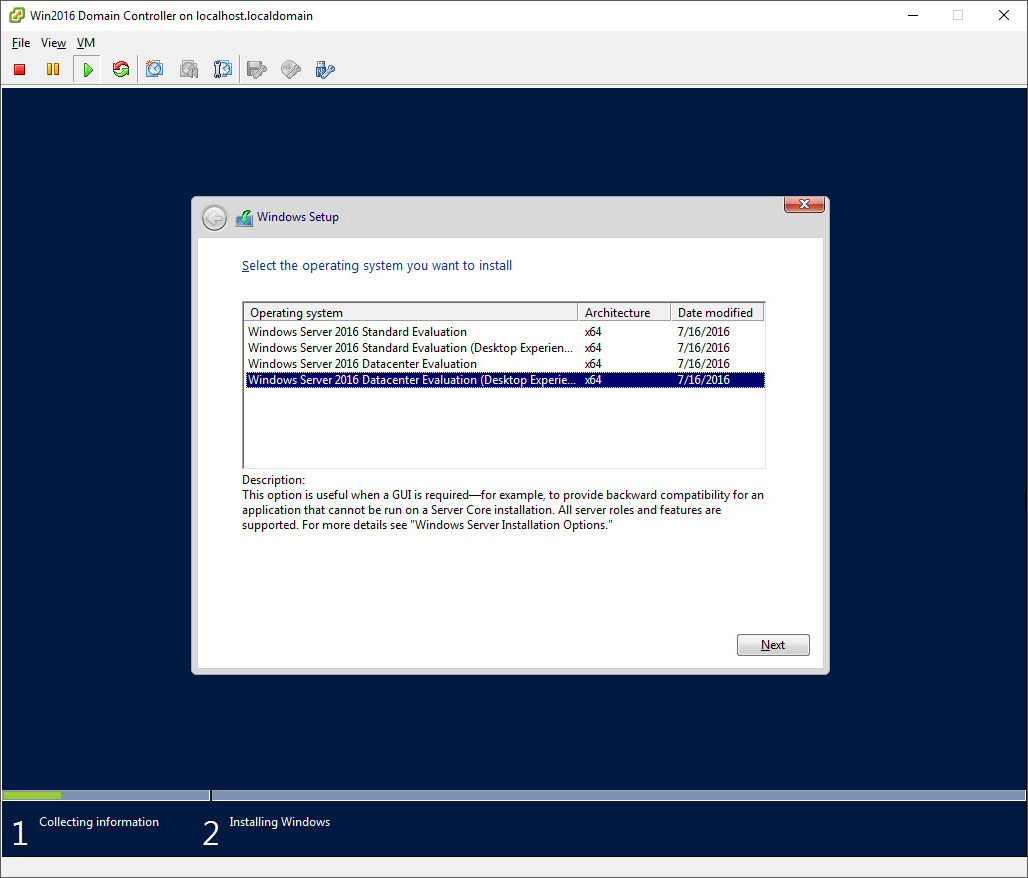
\includegraphics[width=\textwidth]{task2_6_winserver2016_15_dc}
          \caption{Choosing `Datacenter Evaluation (Desktop Experience)'}
          \label{fig:task2:vspherec_windc1}
        \end{figure}
      \item Selecting a strong password for the administrative user. Below I have included a screenshot that shows the warning displayed in the event that the password provided does not meet the minimum complexity requirements.
        \begin{figure}[H]
          \centering
          \captionsetup{skip=2pt}
          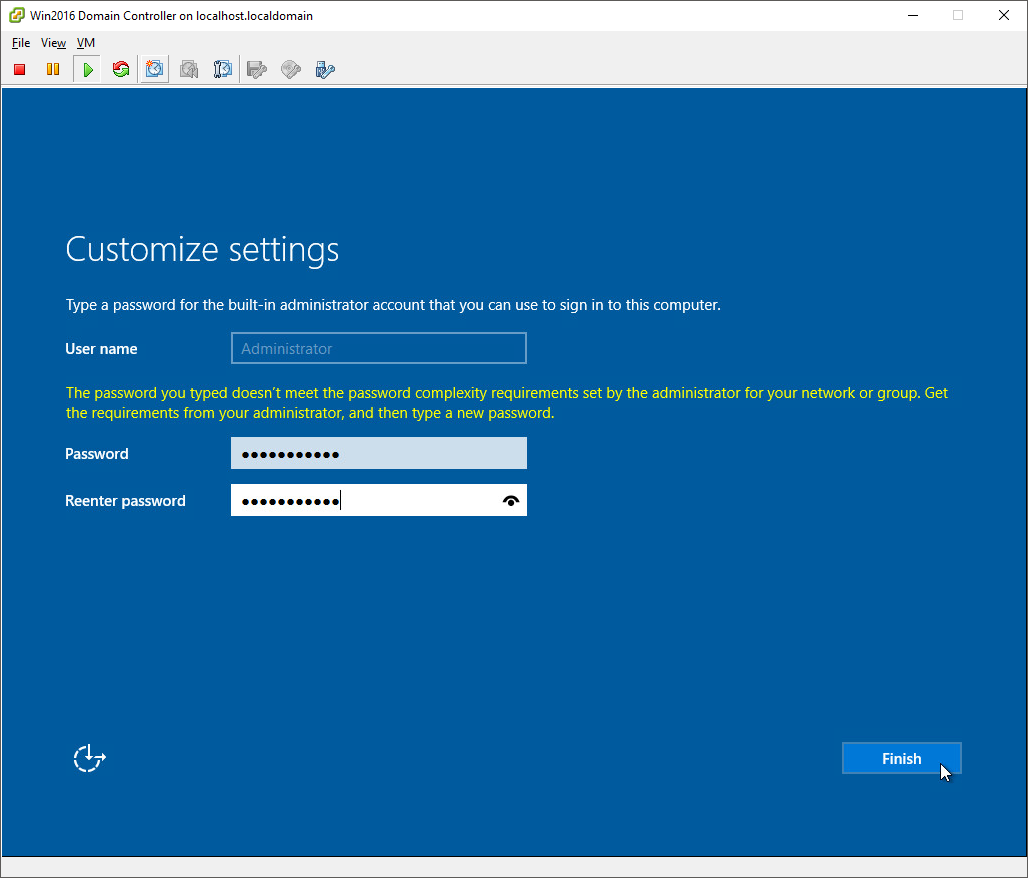
\includegraphics[width=\textwidth]{task2_6_winserver2016_21_dc}
          \caption{Warning message displayed if password does not meet complexity requirements}
          \label{fig:task2:vspherec_windc2}
        \end{figure}
    \end{enumerate}
\end{enumerate}

\noindent \todo{add stuff here about fixing the NAT with ESXi? and changing the hostname}

\subsubsection{Configure an Active Directory Domain Controller}
\begin{enumerate}[series=task2methodology3]
  \item Login to the Domain Controller server and in `Server Manager > Dashboard' select `Add roles and features'.
  \item Proceed through the `Add Roles and Features Wizard' as detailed in the following steps:
   \begin{enumerate}[label=(\alph*)]
     \item \todo{Select configure role-based...}
       \begin{figure}[H]
         \centering
         \captionsetup{skip=2pt}
         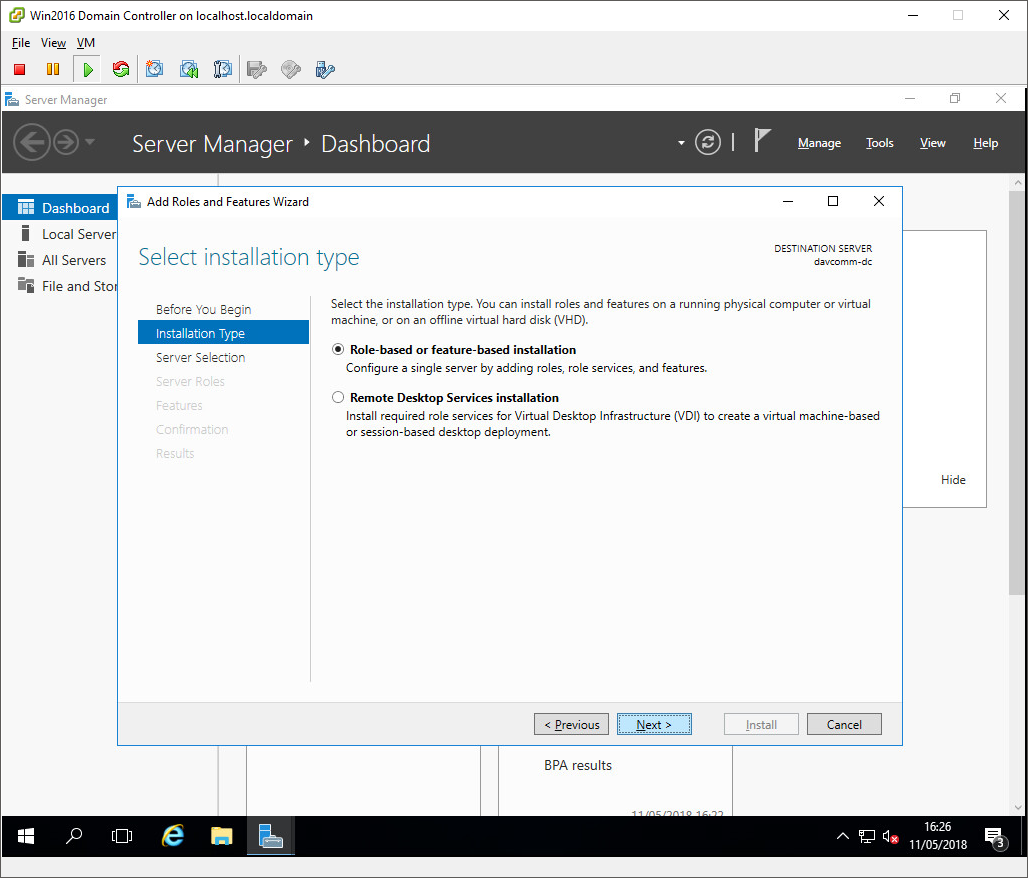
\includegraphics[width=\textwidth]{task2_6_winserver2016_25_dc_config_3}
         \caption{\todo{replace this with a proper figure description}}
         \label{fig:task2:vspherec_windc2_c3}
       \end{figure}
      \item \todo{Select destination server...}
        \begin{figure}[H]
          \centering
          \captionsetup{skip=2pt}
          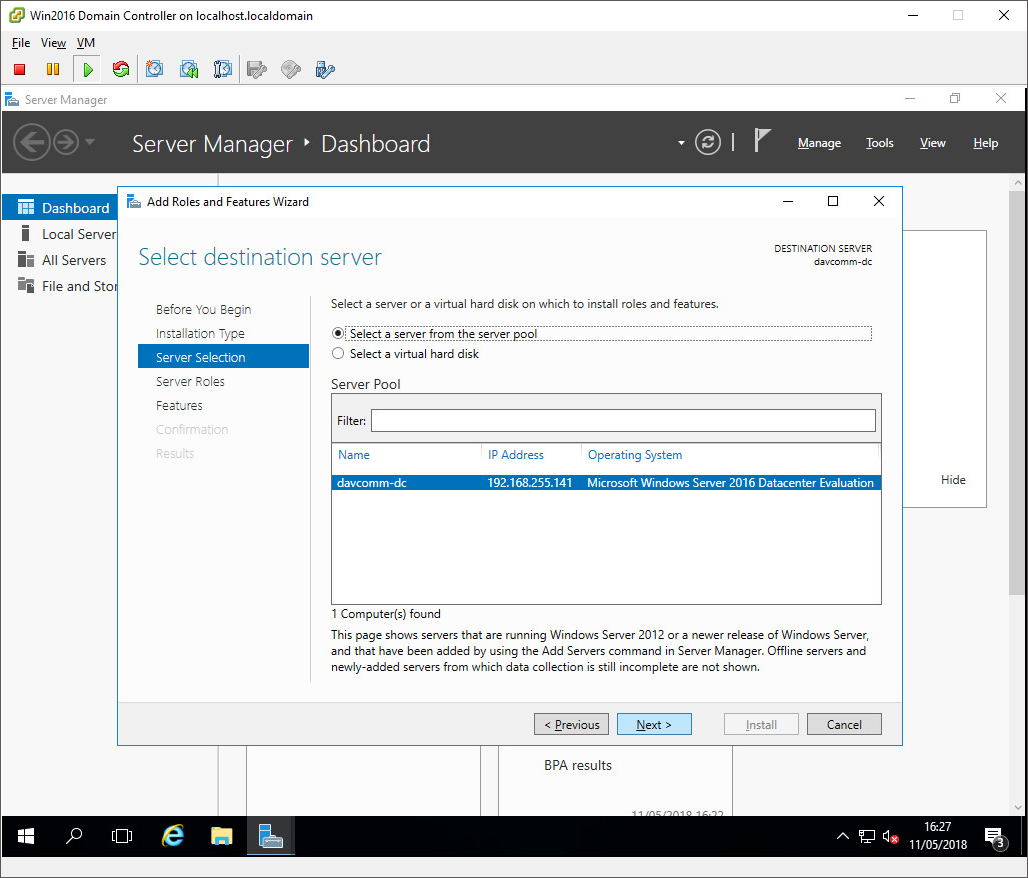
\includegraphics[width=\textwidth]{task2_6_winserver2016_25_dc_config_4}
          \caption{\todo{replace this with a proper figure description}}
          \label{fig:task2:vspherec_windc2_c4}
        \end{figure}
      \item \todo{Add features for ADDS and DNS}
        \begin{figure}[H]
          \centering
          \captionsetup{skip=2pt}
          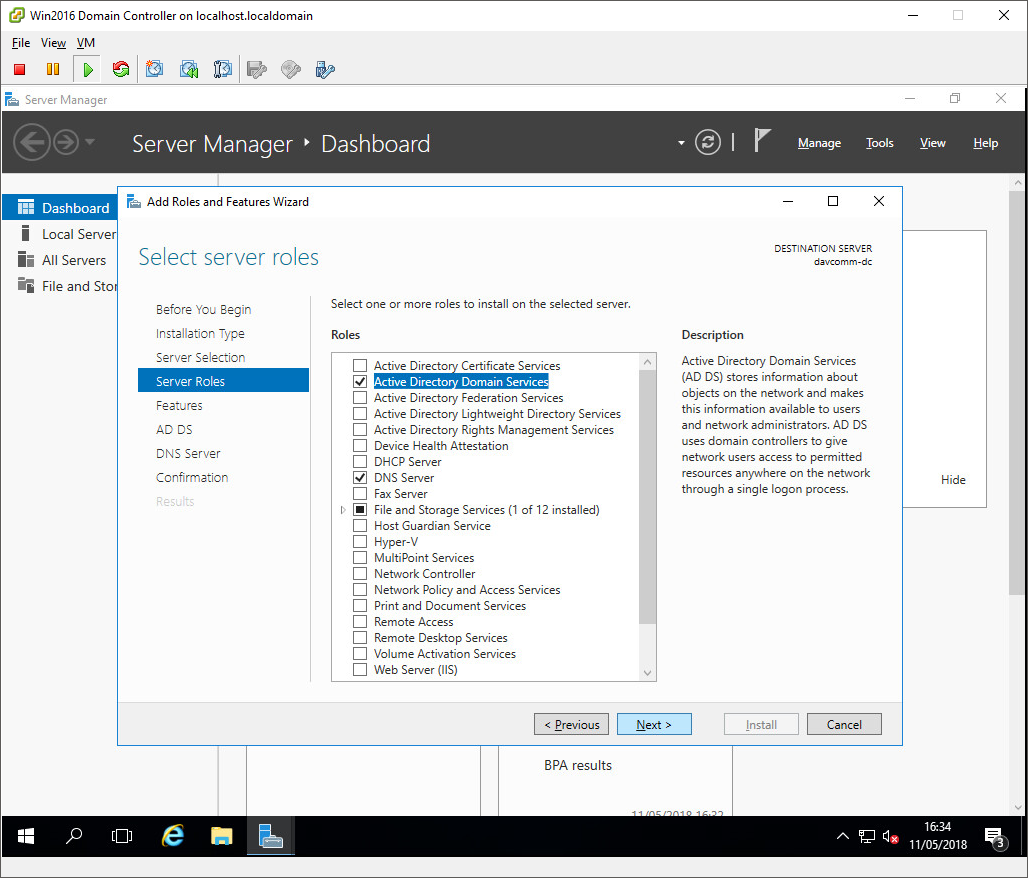
\includegraphics[width=\textwidth]{task2_6_winserver2016_25_dc_config_7}
          \caption{\todo{replace this with a proper figure description}}
          \label{fig:task2:vspherec_windc2_c7}
        \end{figure}
        \begin{figure}[H]
          \centering
          \captionsetup{skip=2pt}
          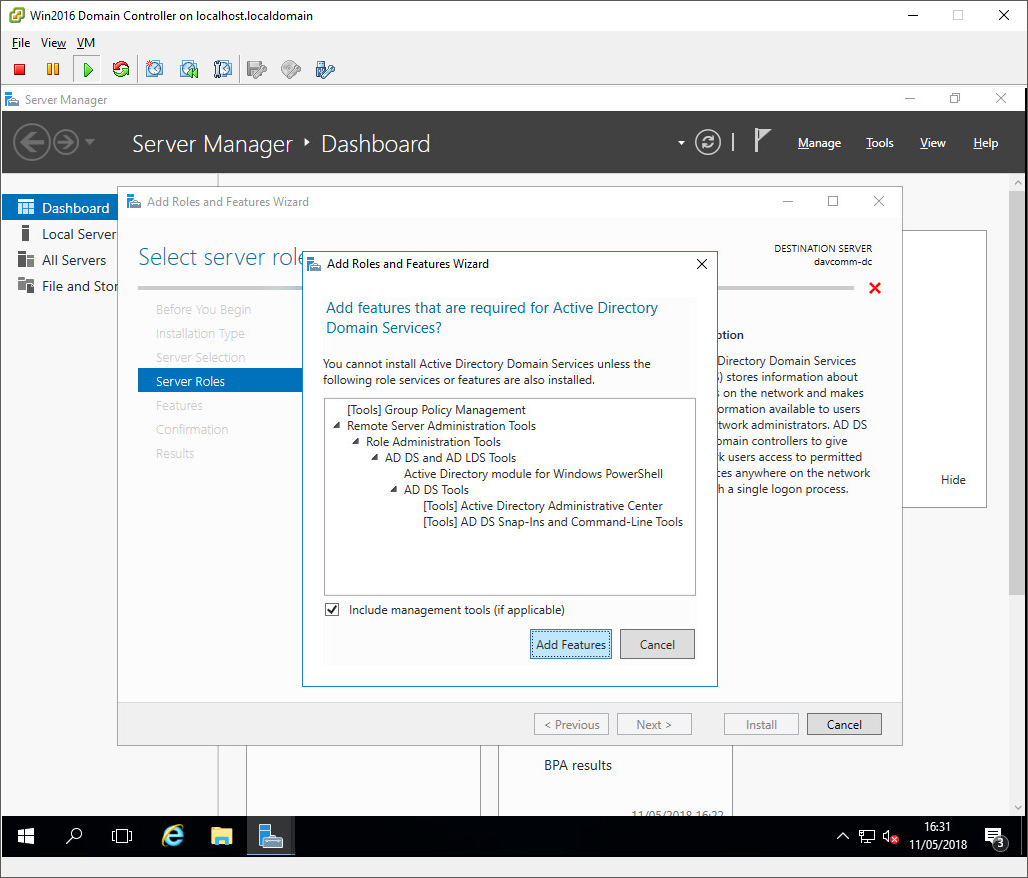
\includegraphics[width=\textwidth]{task2_6_winserver2016_25_dc_config_5}
          \caption{\todo{replace this with a proper figure description}}
          \label{fig:task2:vspherec_windc2_c5}
        \end{figure}
        \begin{figure}[H]
          \centering
          \captionsetup{skip=2pt}
          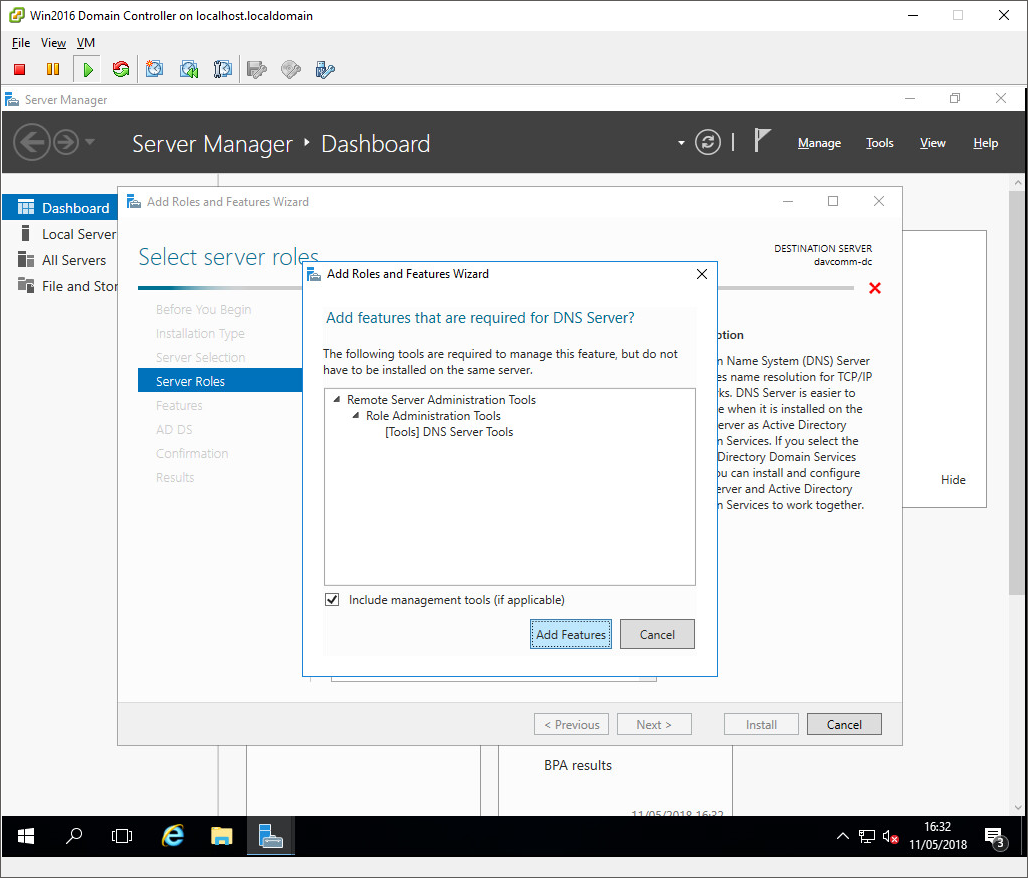
\includegraphics[width=\textwidth]{task2_6_winserver2016_25_dc_config_6}
          \caption{\todo{replace this with a proper figure description}}
          \label{fig:task2:vspherec_windc2_c6}
        \end{figure}
      \item \todo{Confirm installation selections...}
        \begin{figure}[H]
          \centering
          \captionsetup{skip=2pt}
          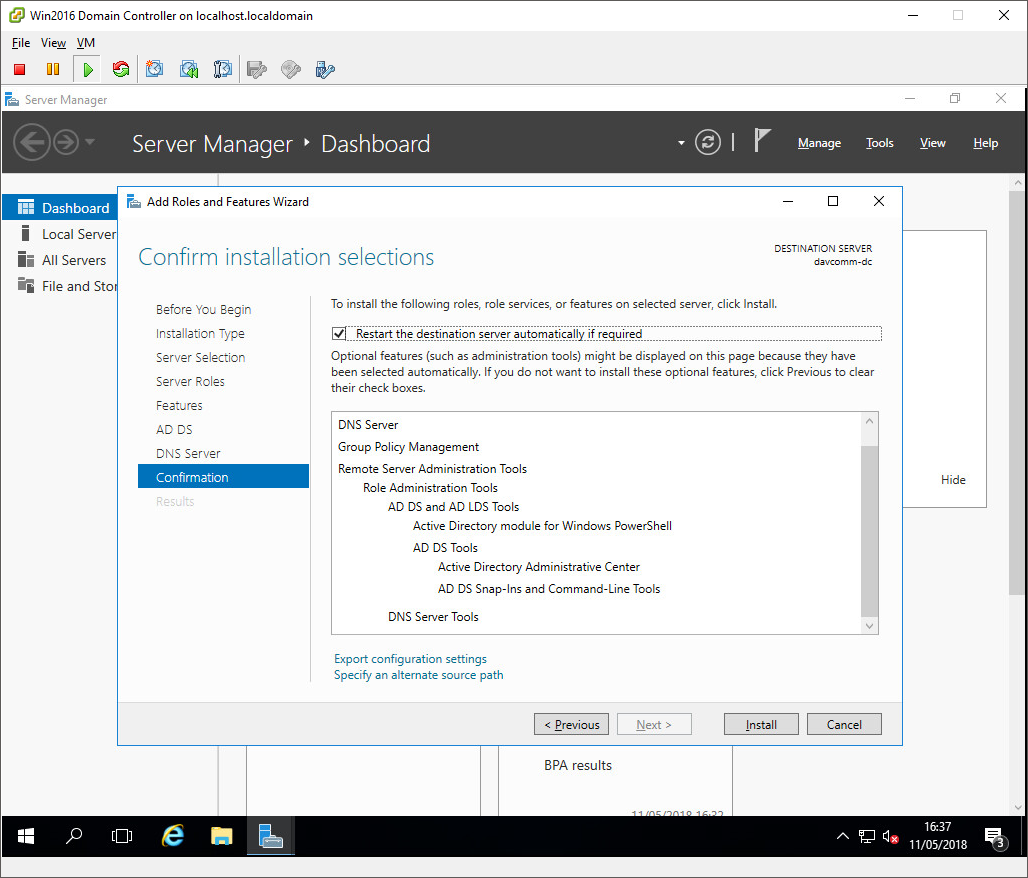
\includegraphics[width=\textwidth]{task2_6_winserver2016_25_dc_config_10}
          \caption{\todo{replace this with a proper figure description}}
          \label{fig:task2:vspherec_windc2_c10}
        \end{figure}
      \item \todo{Create a new forest for the ADDS deployment configuration}
        \begin{figure}[H]
          \centering
          \captionsetup{skip=2pt}
          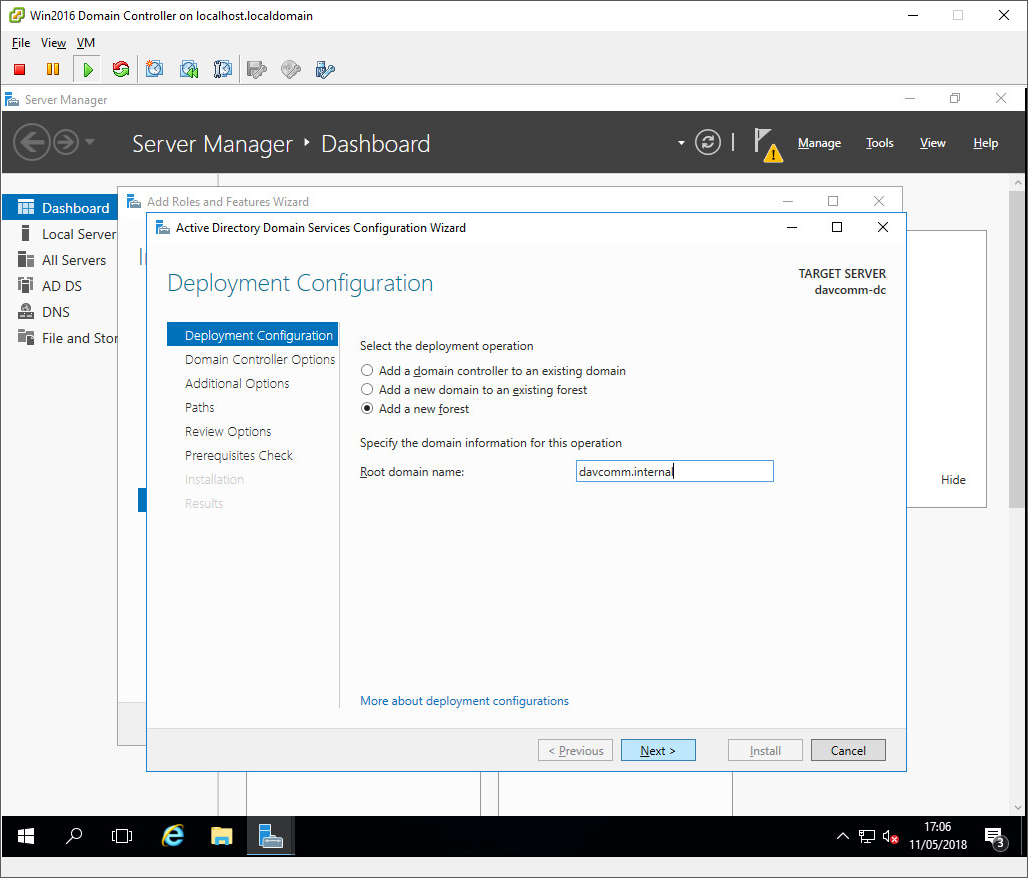
\includegraphics[width=\textwidth]{task2_6_winserver2016_25_dc_config_13}
          \caption{\todo{replace this with a proper figure description}}
          \label{fig:task2:vspherec_windc2_c13}
        \end{figure}
      \item \todo{Set domain controller options...}
        \begin{figure}[H]
          \centering
          \captionsetup{skip=2pt}
          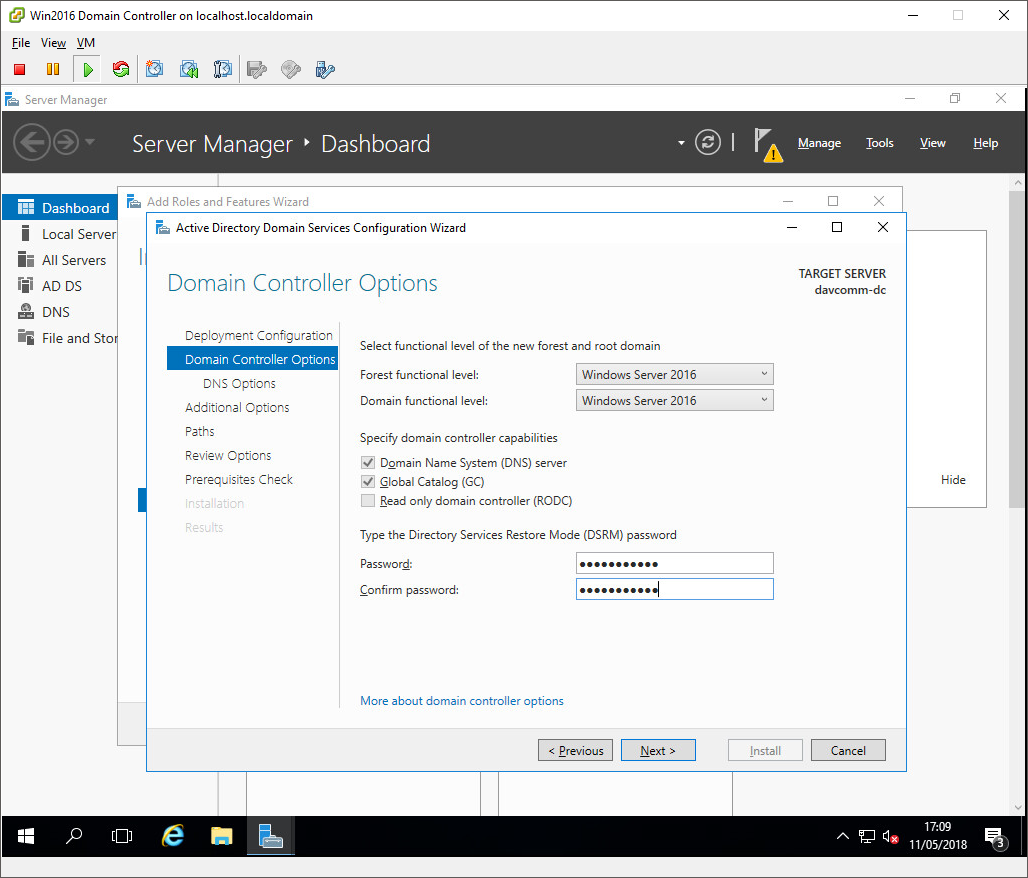
\includegraphics[width=\textwidth]{task2_6_winserver2016_25_dc_config_14}
          \caption{\todo{replace this with a proper figure description}}
          \label{fig:task2:vspherec_windc2_c14}
        \end{figure}
      \item \todo{skip this step - it's fine xd}
        \begin{figure}[H]
          \centering
          \captionsetup{skip=2pt}
          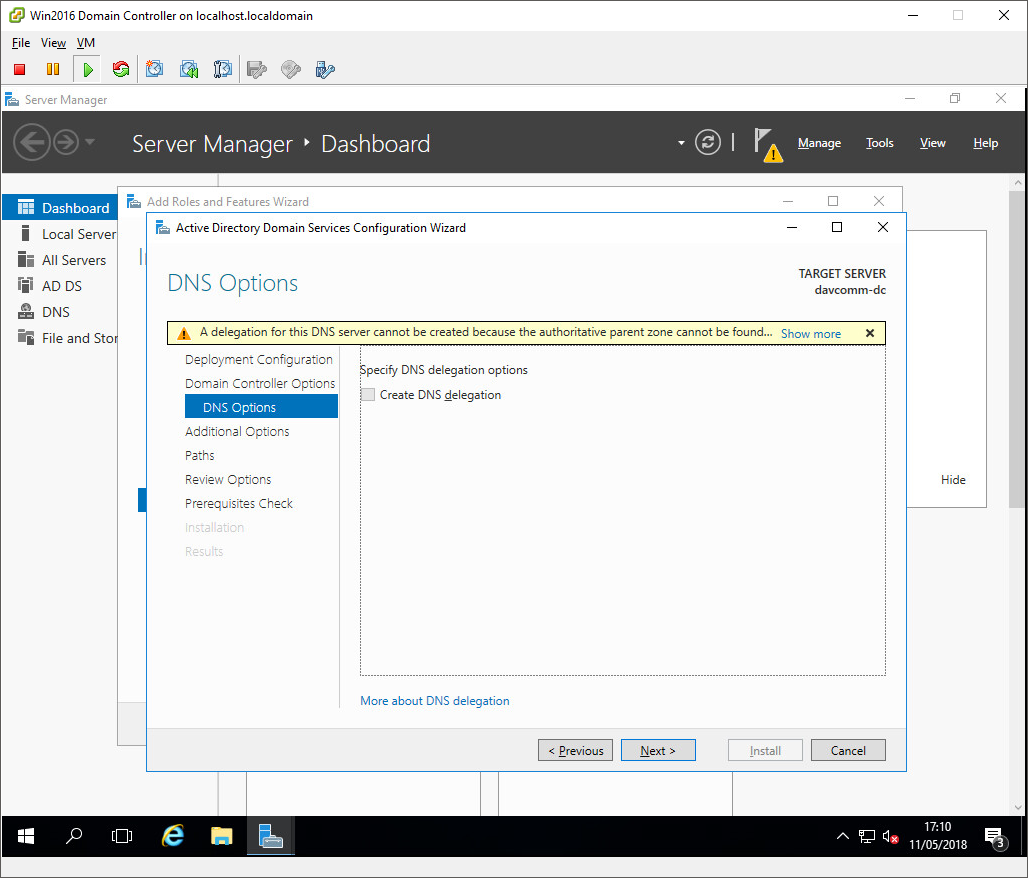
\includegraphics[width=\textwidth]{task2_6_winserver2016_25_dc_config_15}
          \caption{\todo{replace this with a proper figure description}}
          \label{fig:task2:vspherec_windc2_c15}
        \end{figure}
      \item \todo{Set the NetBIOS name...}
        \begin{figure}[H]
          \centering
          \captionsetup{skip=2pt}
          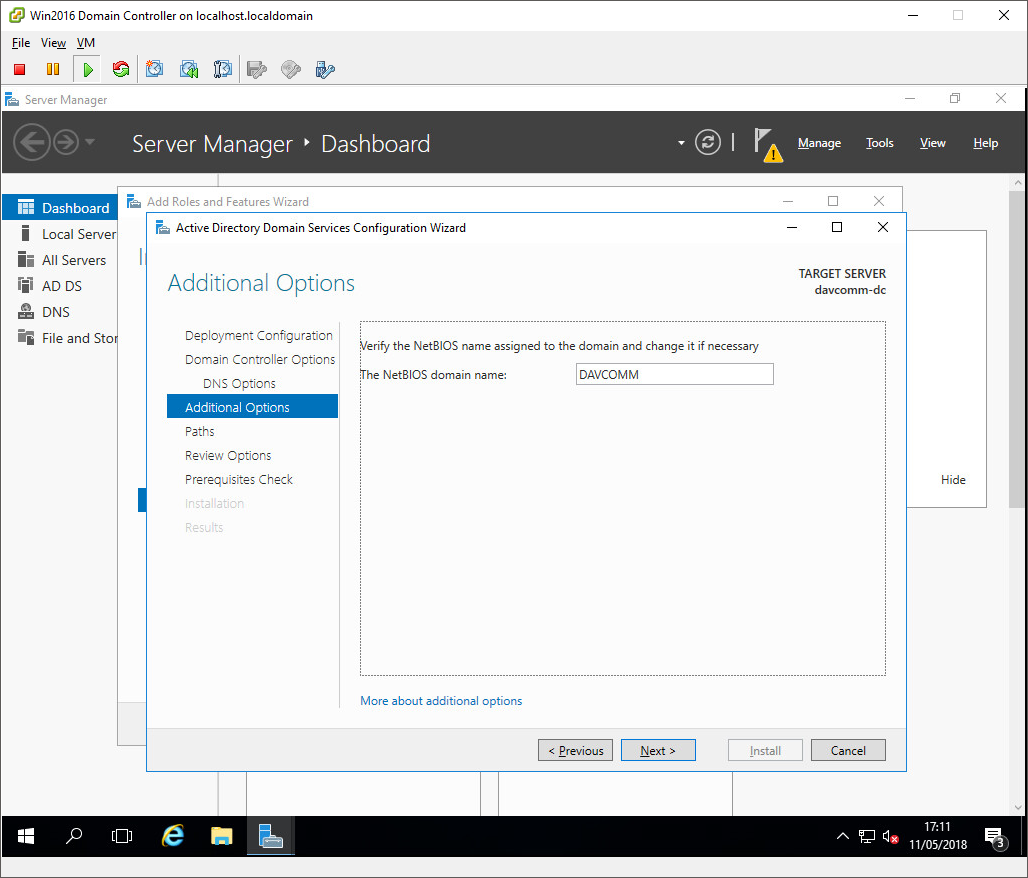
\includegraphics[width=\textwidth]{task2_6_winserver2016_25_dc_config_16}
          \caption{\todo{replace this with a proper figure description}}
          \label{fig:task2:vspherec_windc2_c16}
        \end{figure}
      \item \todo{Leave the defaults for paths here... maybe discuss how we could use remote locations or different partitions for these, especially log files could be a write-once disk}
        \begin{figure}[H]
          \centering
          \captionsetup{skip=2pt}
          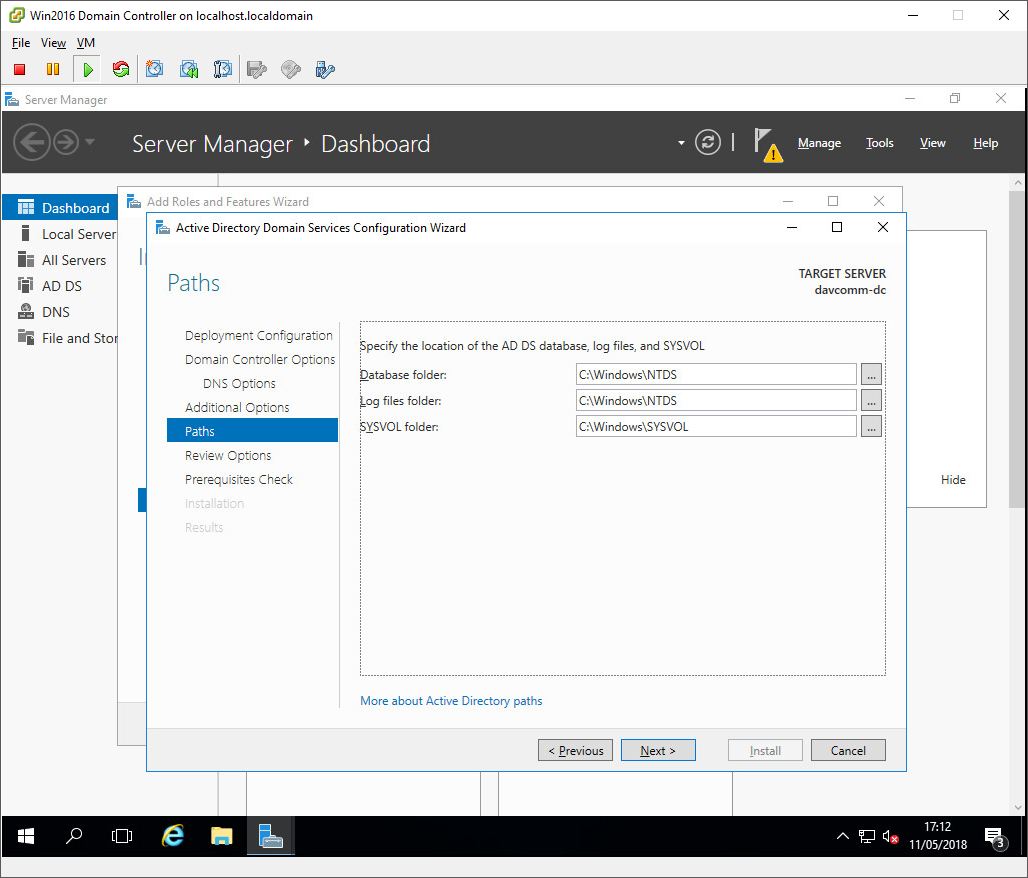
\includegraphics[width=\textwidth]{task2_6_winserver2016_25_dc_config_17}
          \caption{\todo{replace this with a proper figure description}}
          \label{fig:task2:vspherec_windc2_c17}
        \end{figure}
      \item \todo{review the options and confirm - note the ability to view the PowerShell script for this configuration, talk about how these deployments could be automated}
        \begin{figure}[H]
          \centering
          \captionsetup{skip=2pt}
          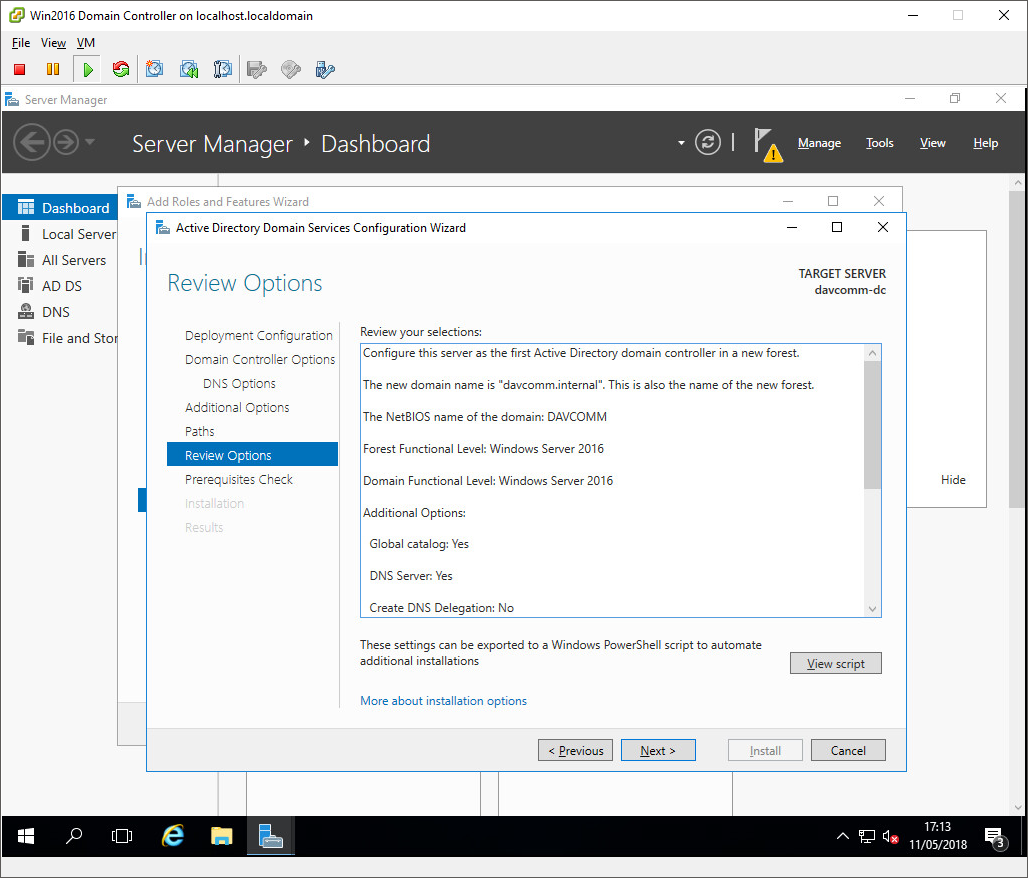
\includegraphics[width=\textwidth]{task2_6_winserver2016_25_dc_config_18}
          \caption{\todo{replace this with a proper figure description}}
          \label{fig:task2:vspherec_windc2_c18}
        \end{figure}
        \begin{figure}[H]
          \centering
          \captionsetup{skip=2pt}
          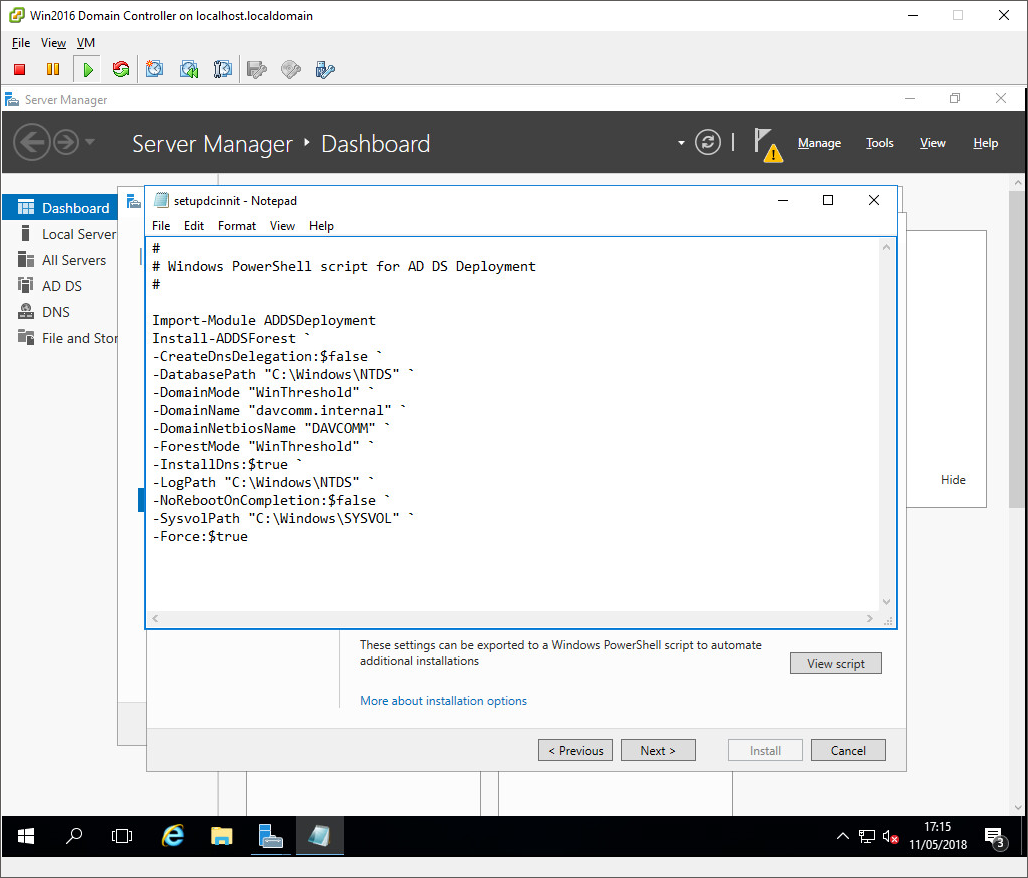
\includegraphics[width=\textwidth]{task2_6_winserver2016_25_dc_config_19}
          \caption{\todo{replace this with a proper figure description}}
          \label{fig:task2:vspherec_windc2_c19}
        \end{figure}
      \item \todo{prereq check - only warnings it is fine}
        \begin{figure}[H]
          \centering
          \captionsetup{skip=2pt}
          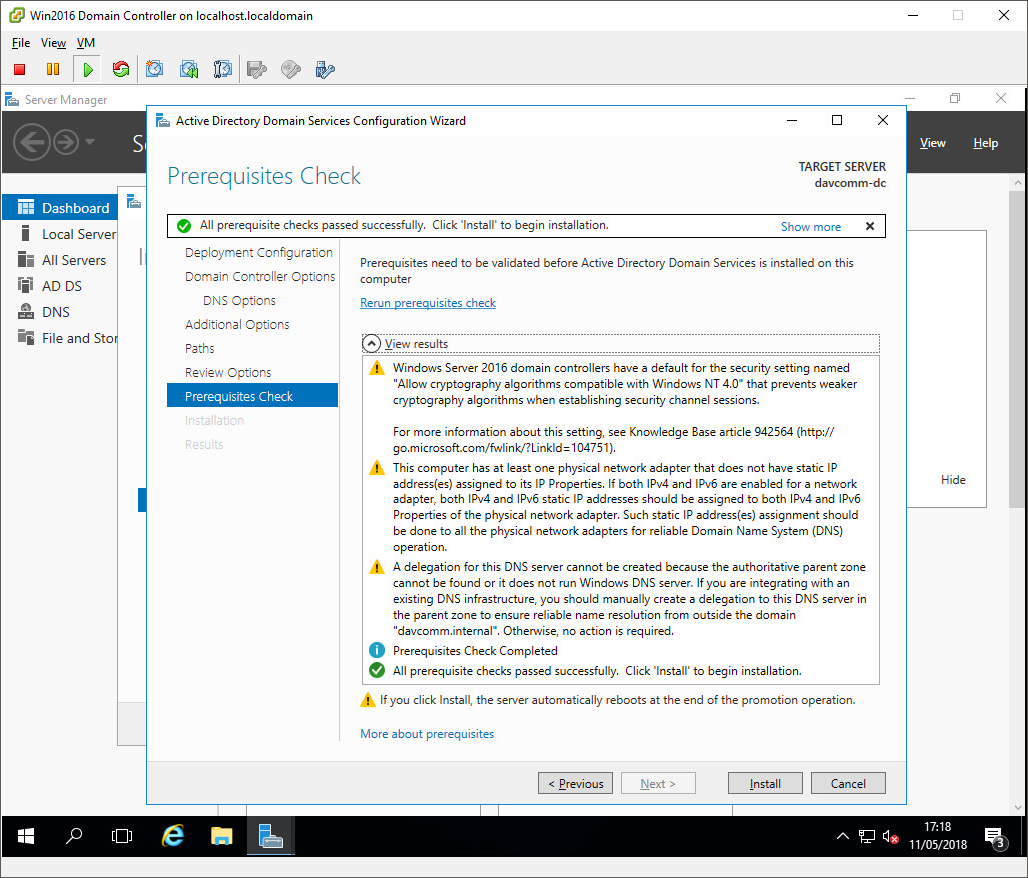
\includegraphics[width=\textwidth]{task2_6_winserver2016_25_dc_config_20}
          \caption{\todo{replace this with a proper figure description}}
          \label{fig:task2:vspherec_windc2_c20}
        \end{figure}
      \item \todo{the server will restart after the role installation, log into the new domain as administrator when you the system has completed restart}
        \begin{figure}[H]
          \centering
          \captionsetup{skip=2pt}
          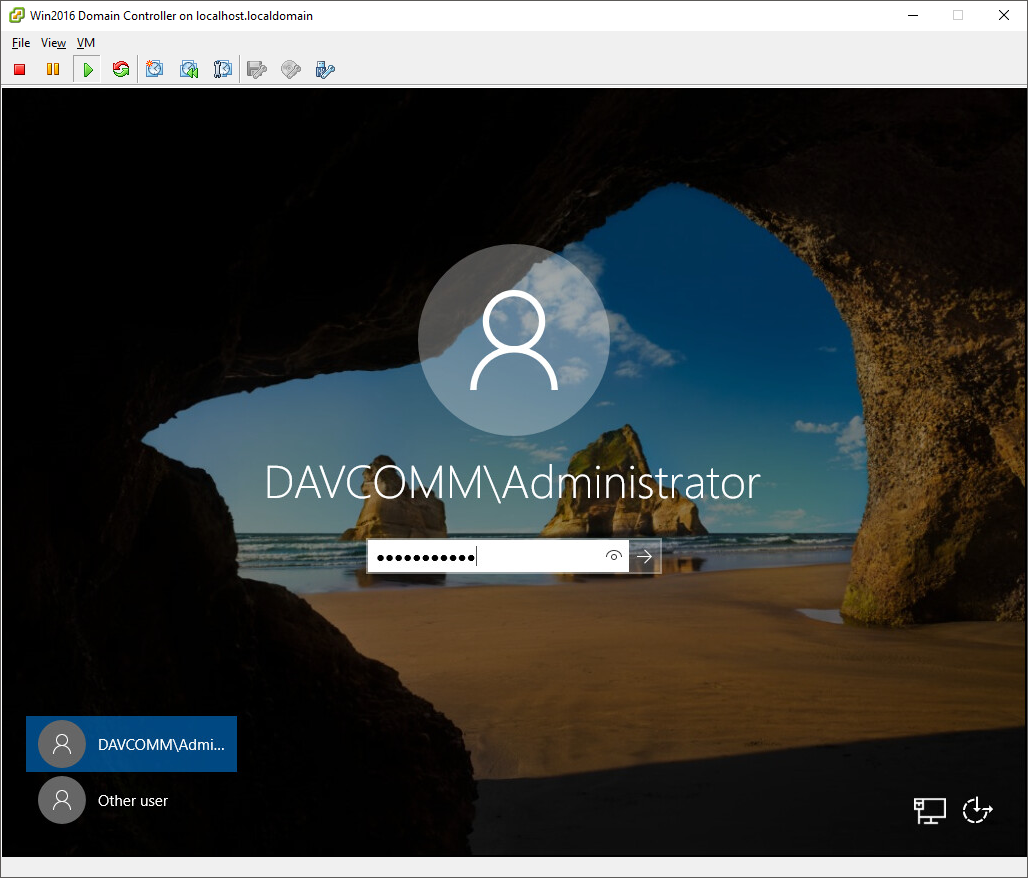
\includegraphics[width=\textwidth]{task2_6_winserver2016_25_dc_config_21}
          \caption{\todo{replace this with a proper figure description}}
          \label{fig:task2:vspherec_windc2_c21}
        \end{figure}
      \item \todo{check the dns is configured correctly to point to self (127.0.0.1) and also make the IP address static, yada yada}
        \begin{figure}[H]
          \centering
          \captionsetup{skip=2pt}
          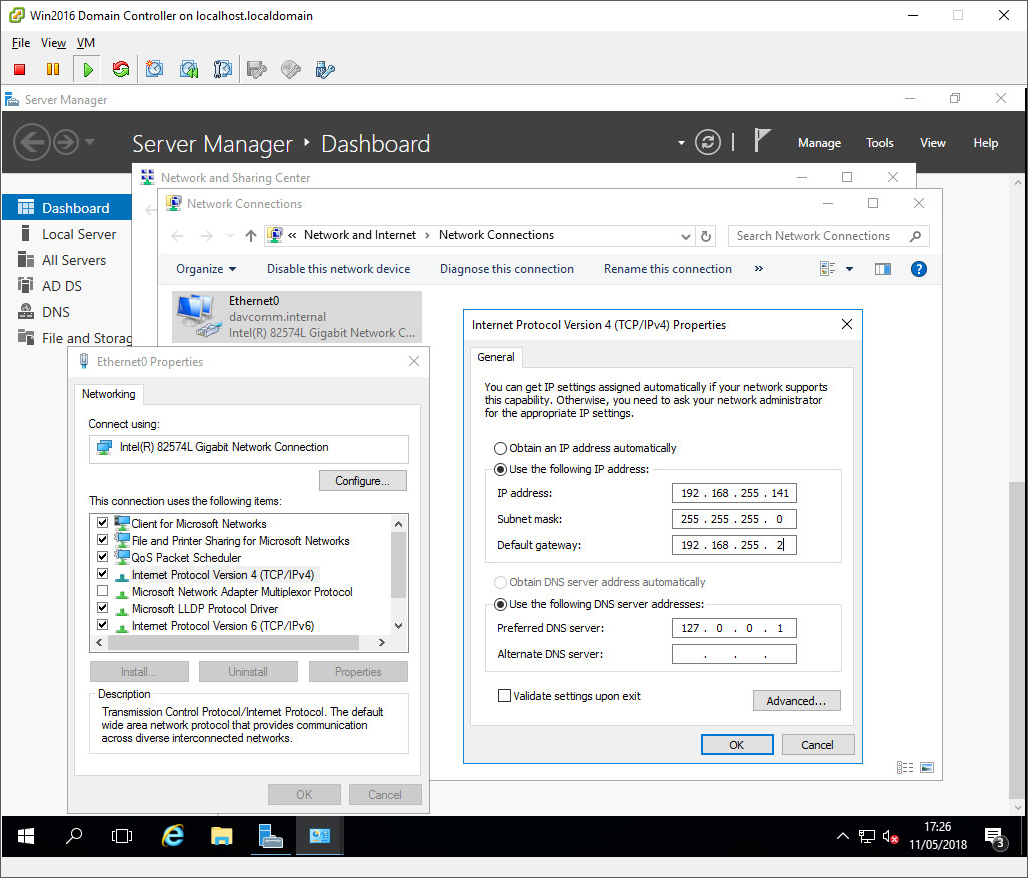
\includegraphics[width=\textwidth]{task2_6_winserver2016_25_dc_config_22_adjustipdns}
          \caption{\todo{replace this with a proper figure description}}
          \label{fig:task2:vspherec_windc2_c22}
        \end{figure}
   \end{enumerate}
\end{enumerate}


\subsubsection{Set up a User Server}
\todo{set up the user server in a similar fashion, i won't repeat the entire process here}
\begin{enumerate}[series=task2methodology4]
  \item \todo{set up vm in esxi web ui}
    \begin{figure}[H]
      \centering
      \captionsetup{skip=2pt}
      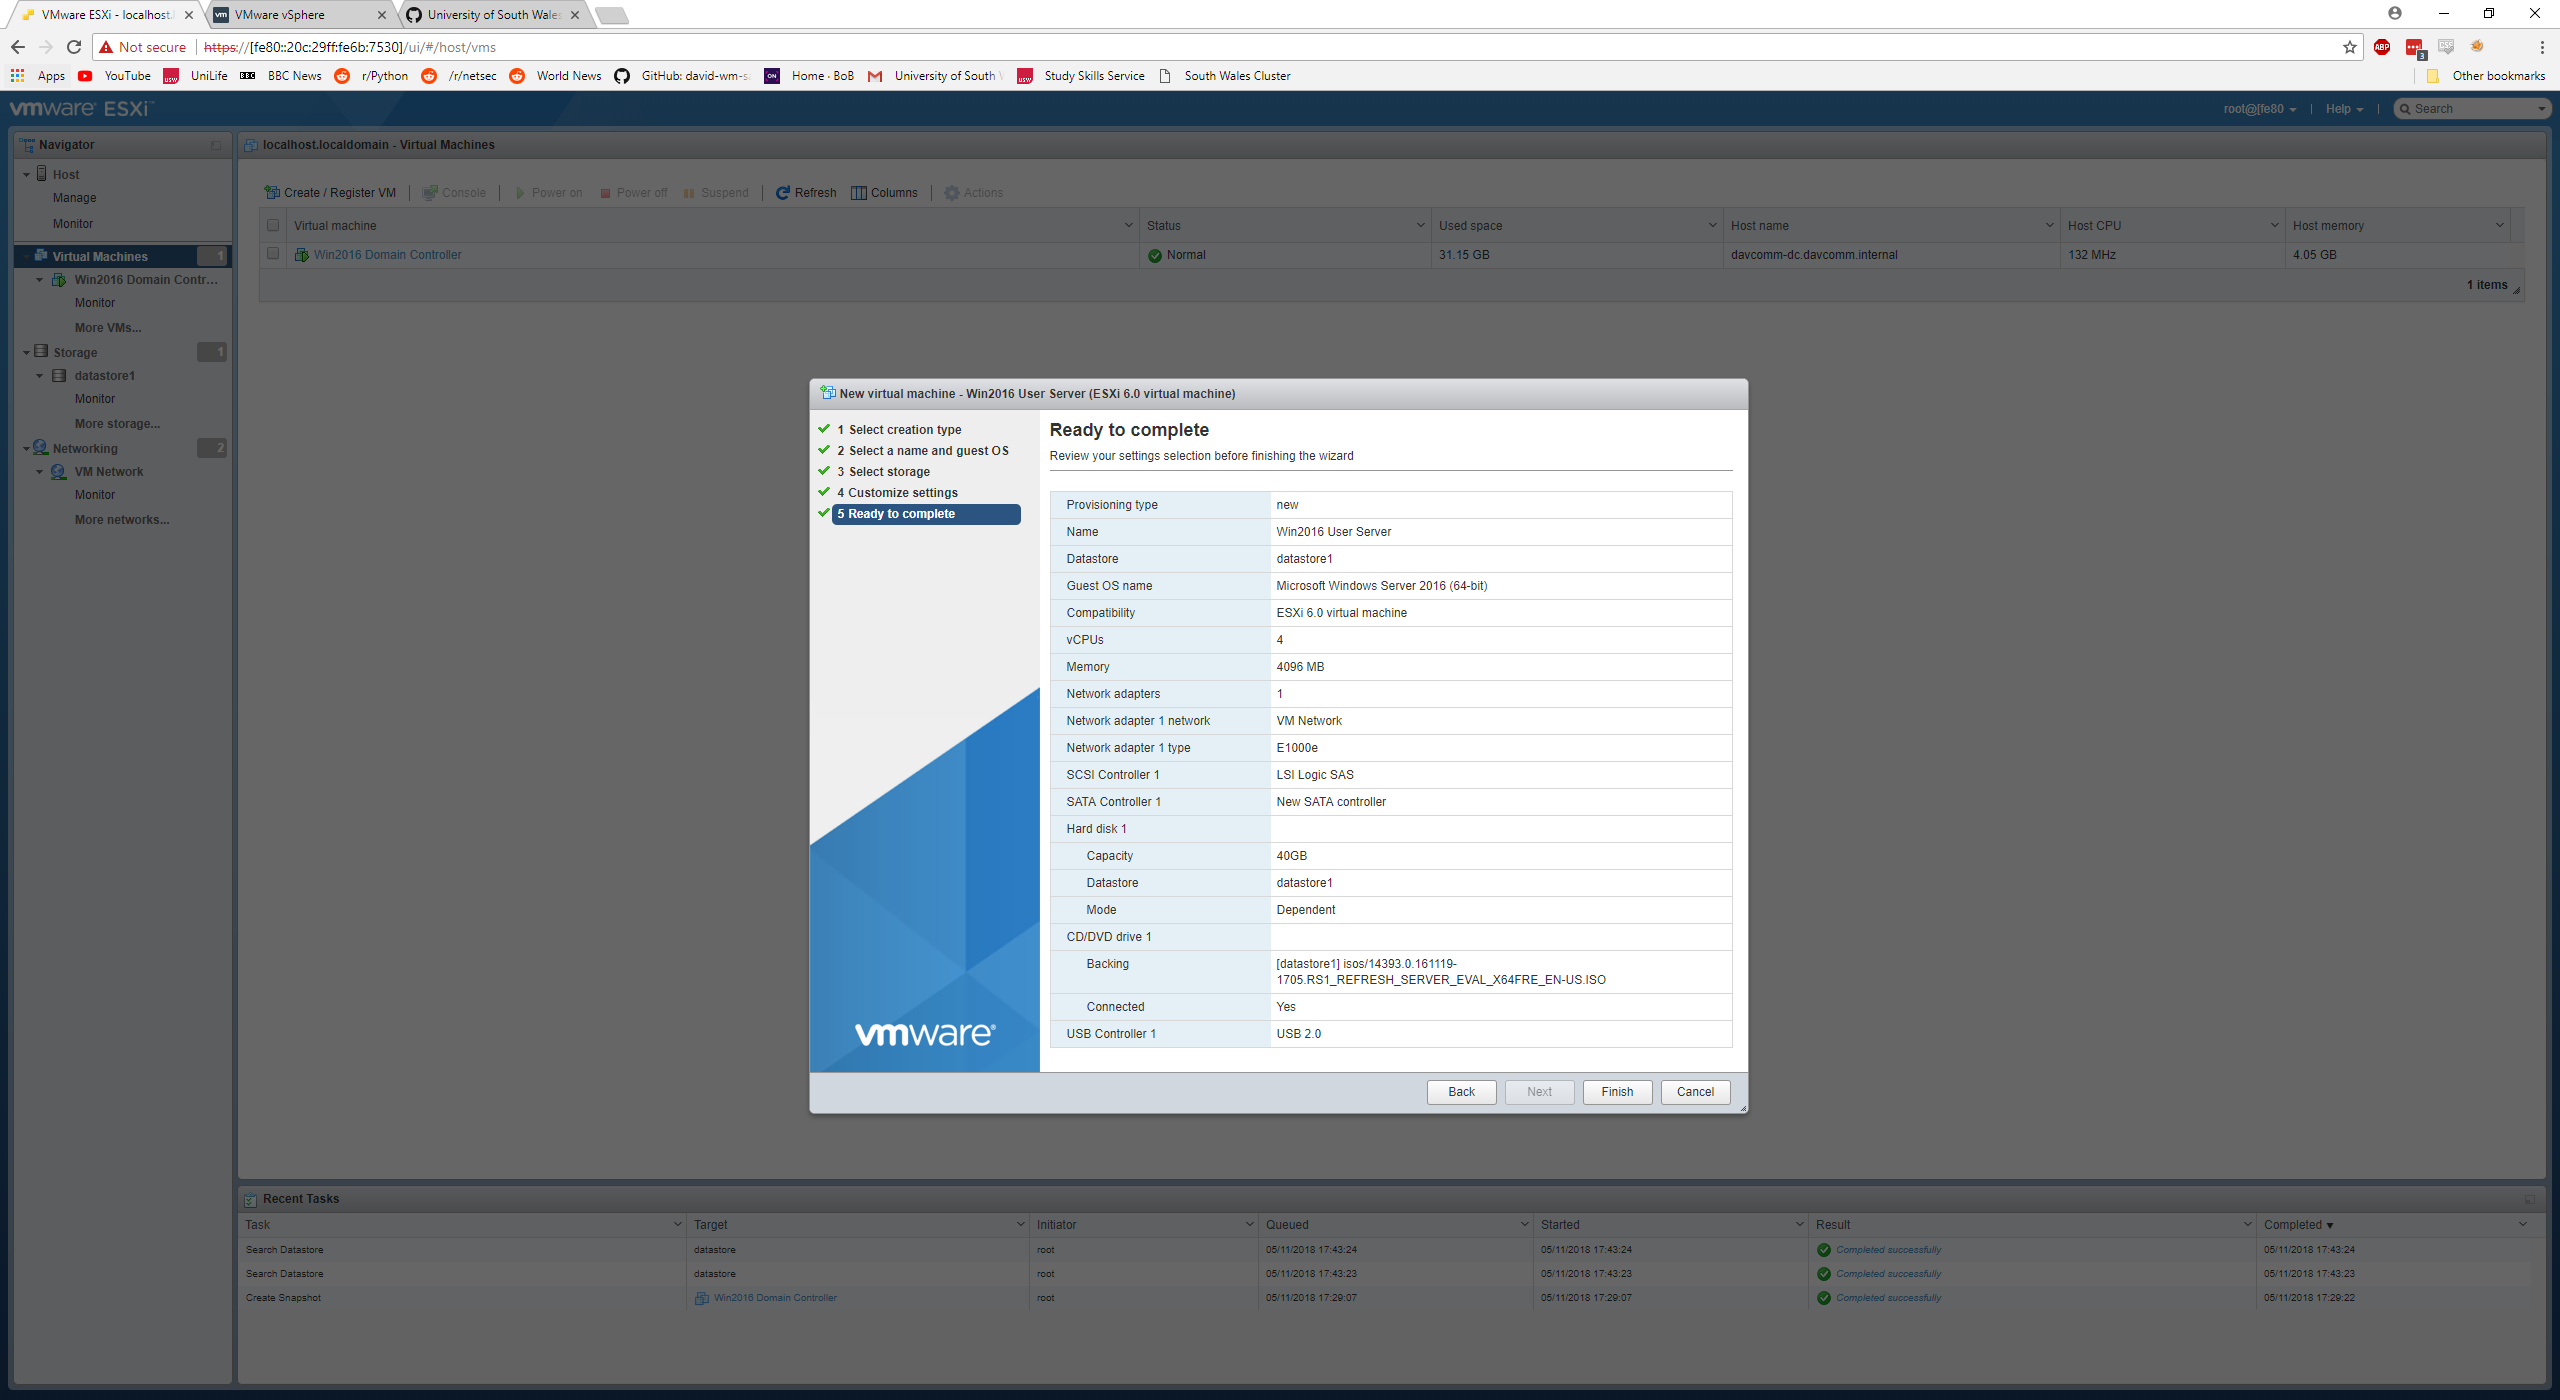
\includegraphics[width=\textwidth]{task2_9_winserver2016us_1}
      \caption{\todo{replace this with a proper figure description}}
      \label{fig:task2:vspherec_us1}
    \end{figure}
  \item \todo{after install point the dns to the static ip of the dc}
    \begin{figure}[H]
      \centering
      \captionsetup{skip=2pt}
      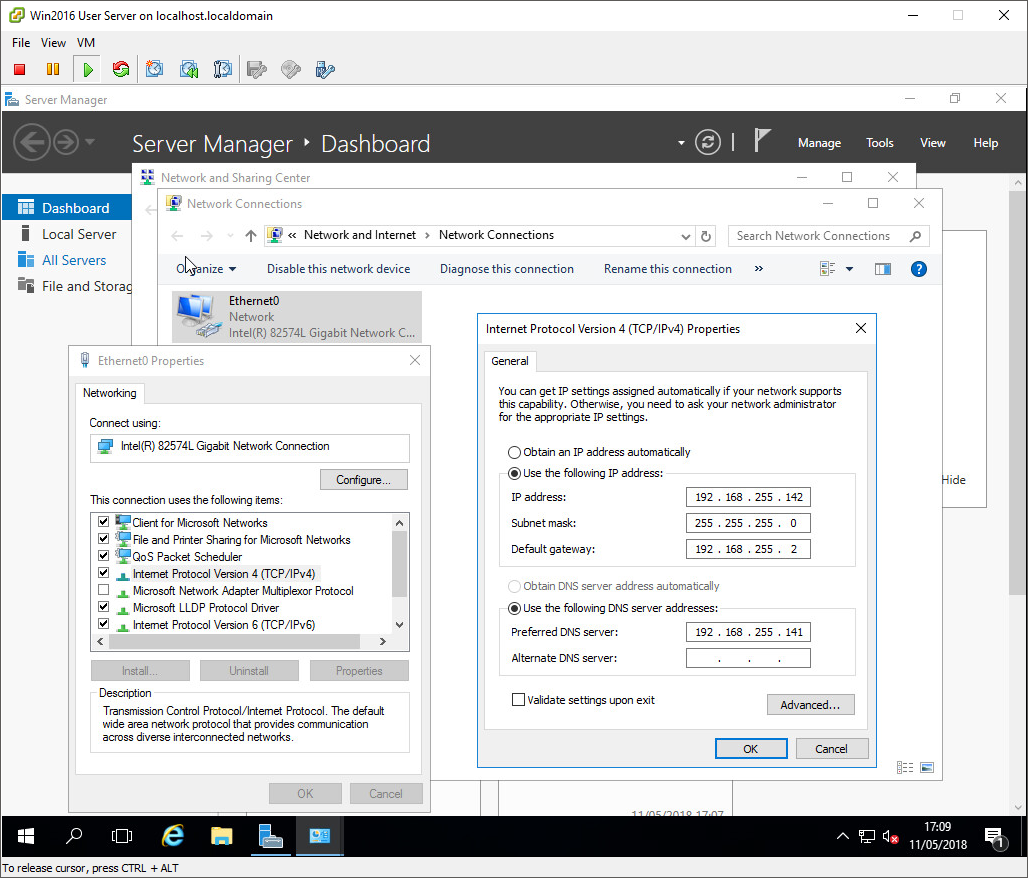
\includegraphics[width=\textwidth]{task2_9_winserver2016us_2}
      \caption{\todo{replace this with a proper figure description}}
      \label{fig:task2:vspherec_us2}
    \end{figure}
  \item \todo{check that we can ping the dc}
    \begin{figure}[H]
      \centering
      \captionsetup{skip=2pt}
      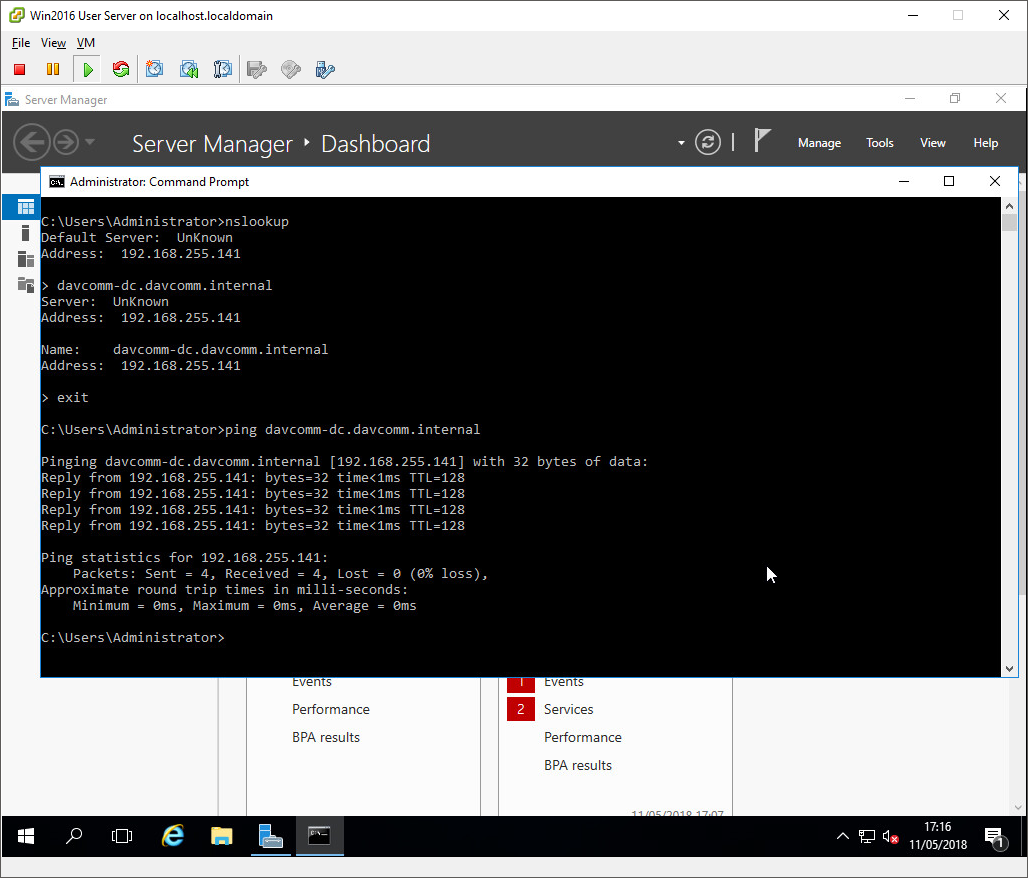
\includegraphics[width=\textwidth]{task2_9_winserver2016us_3}
      \caption{\todo{replace this with a proper figure description}}
      \label{fig:task2:vspherec_us3}
    \end{figure}
  \item \todo{set the hostname and join the domain at the same time}
    \begin{figure}[H]
      \centering
      \captionsetup{skip=2pt}
      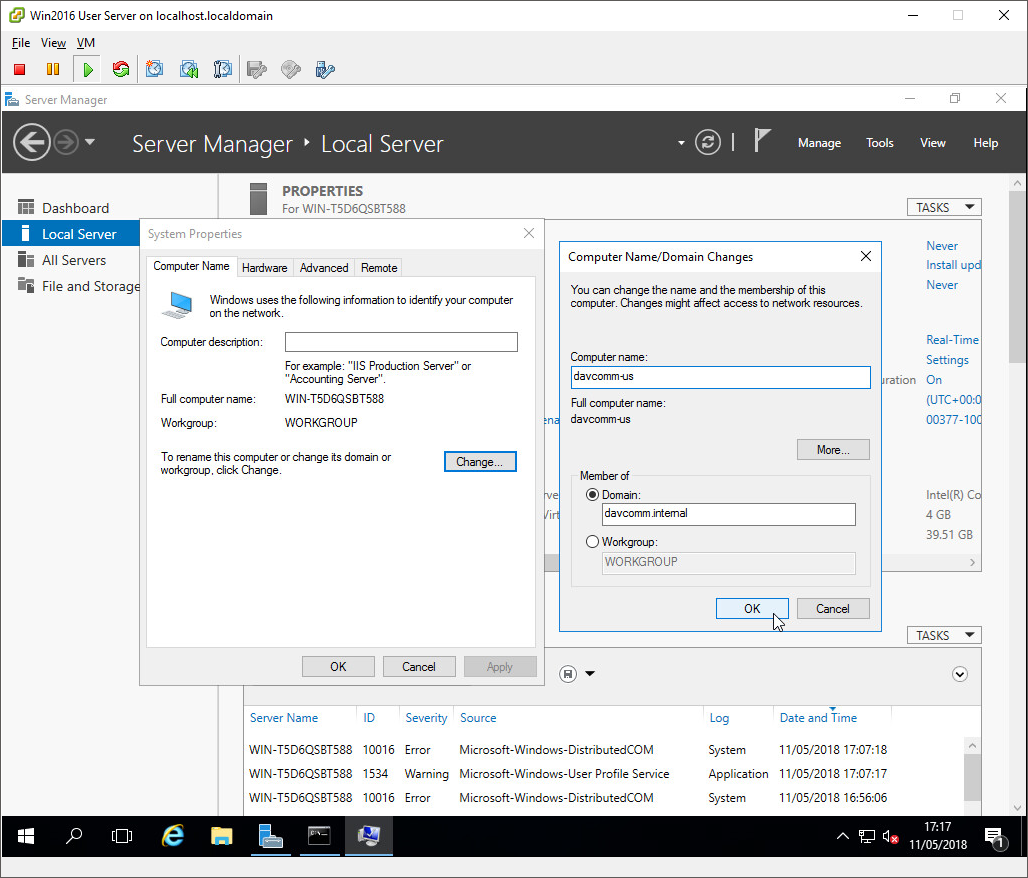
\includegraphics[width=\textwidth]{task2_9_winserver2016us_4}
      \caption{\todo{replace this with a proper figure description}}
      \label{fig:task2:vspherec_us4}
    \end{figure}
  \item \todo{after authenticating with the domain, am welcomed, success}
    \begin{figure}[H]
      \centering
      \captionsetup{skip=2pt}
      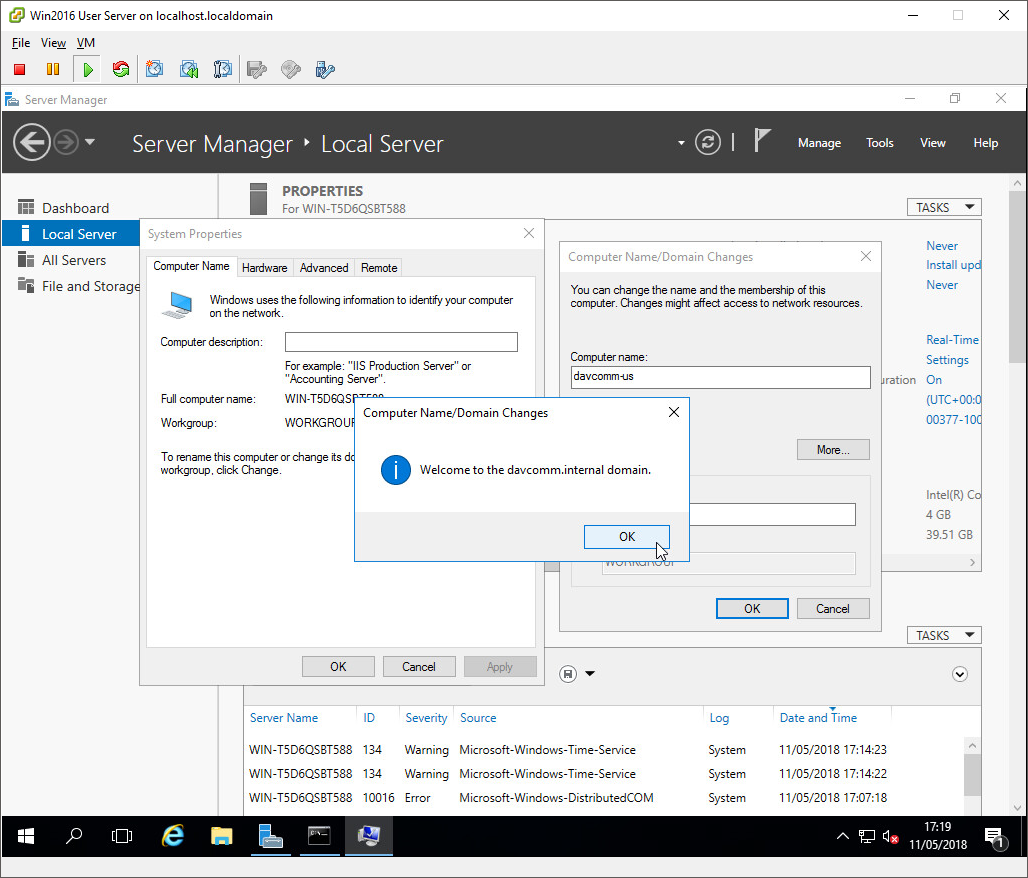
\includegraphics[width=\textwidth]{task2_9_winserver2016us_5}
      \caption{\todo{replace this with a proper figure description}}
      \label{fig:task2:vspherec_us5}
    \end{figure}
  \item \todo{restart to make the changes and login to the domain}
    \begin{figure}[H]
      \centering
      \captionsetup{skip=2pt}
      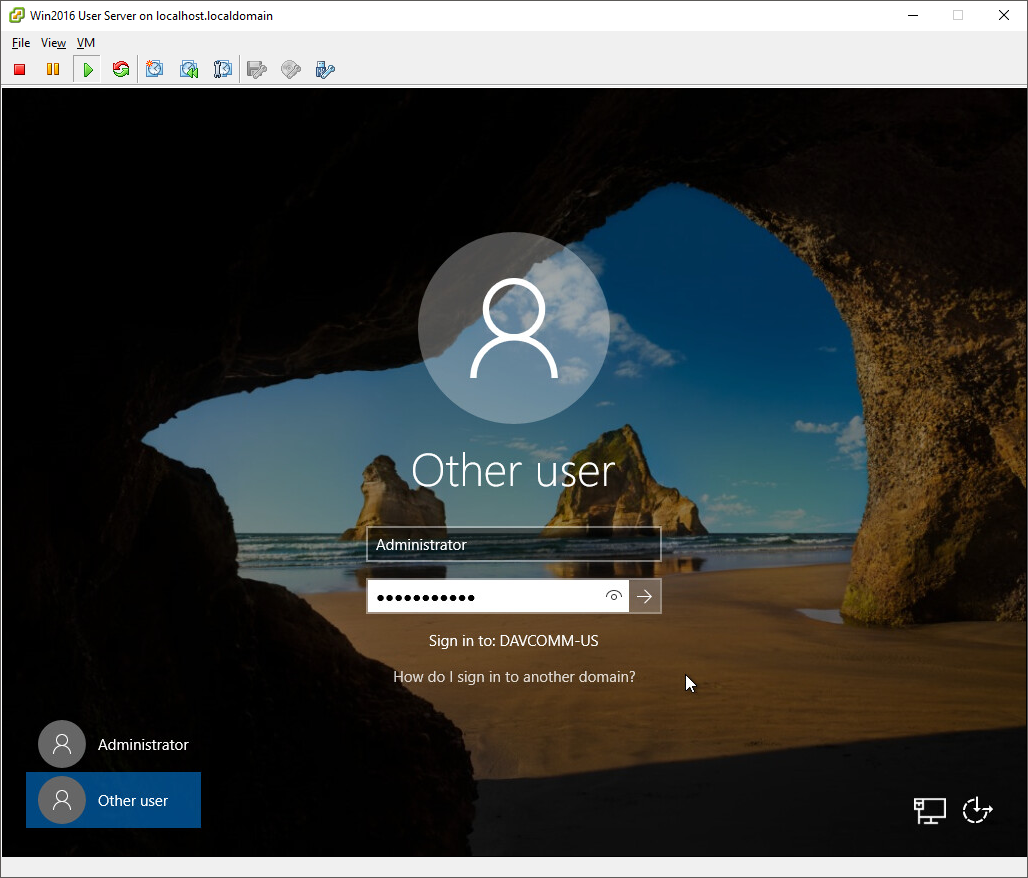
\includegraphics[width=\textwidth]{task2_9_winserver2016us_7}
      \caption{\todo{replace this with a proper figure description}}
      \label{fig:task2:vspherec_us7}
    \end{figure}
  \item \todo{after installing vmware tools we see this in the vsphere webui}
    \begin{figure}[H]
      \centering
      \captionsetup{skip=2pt}
      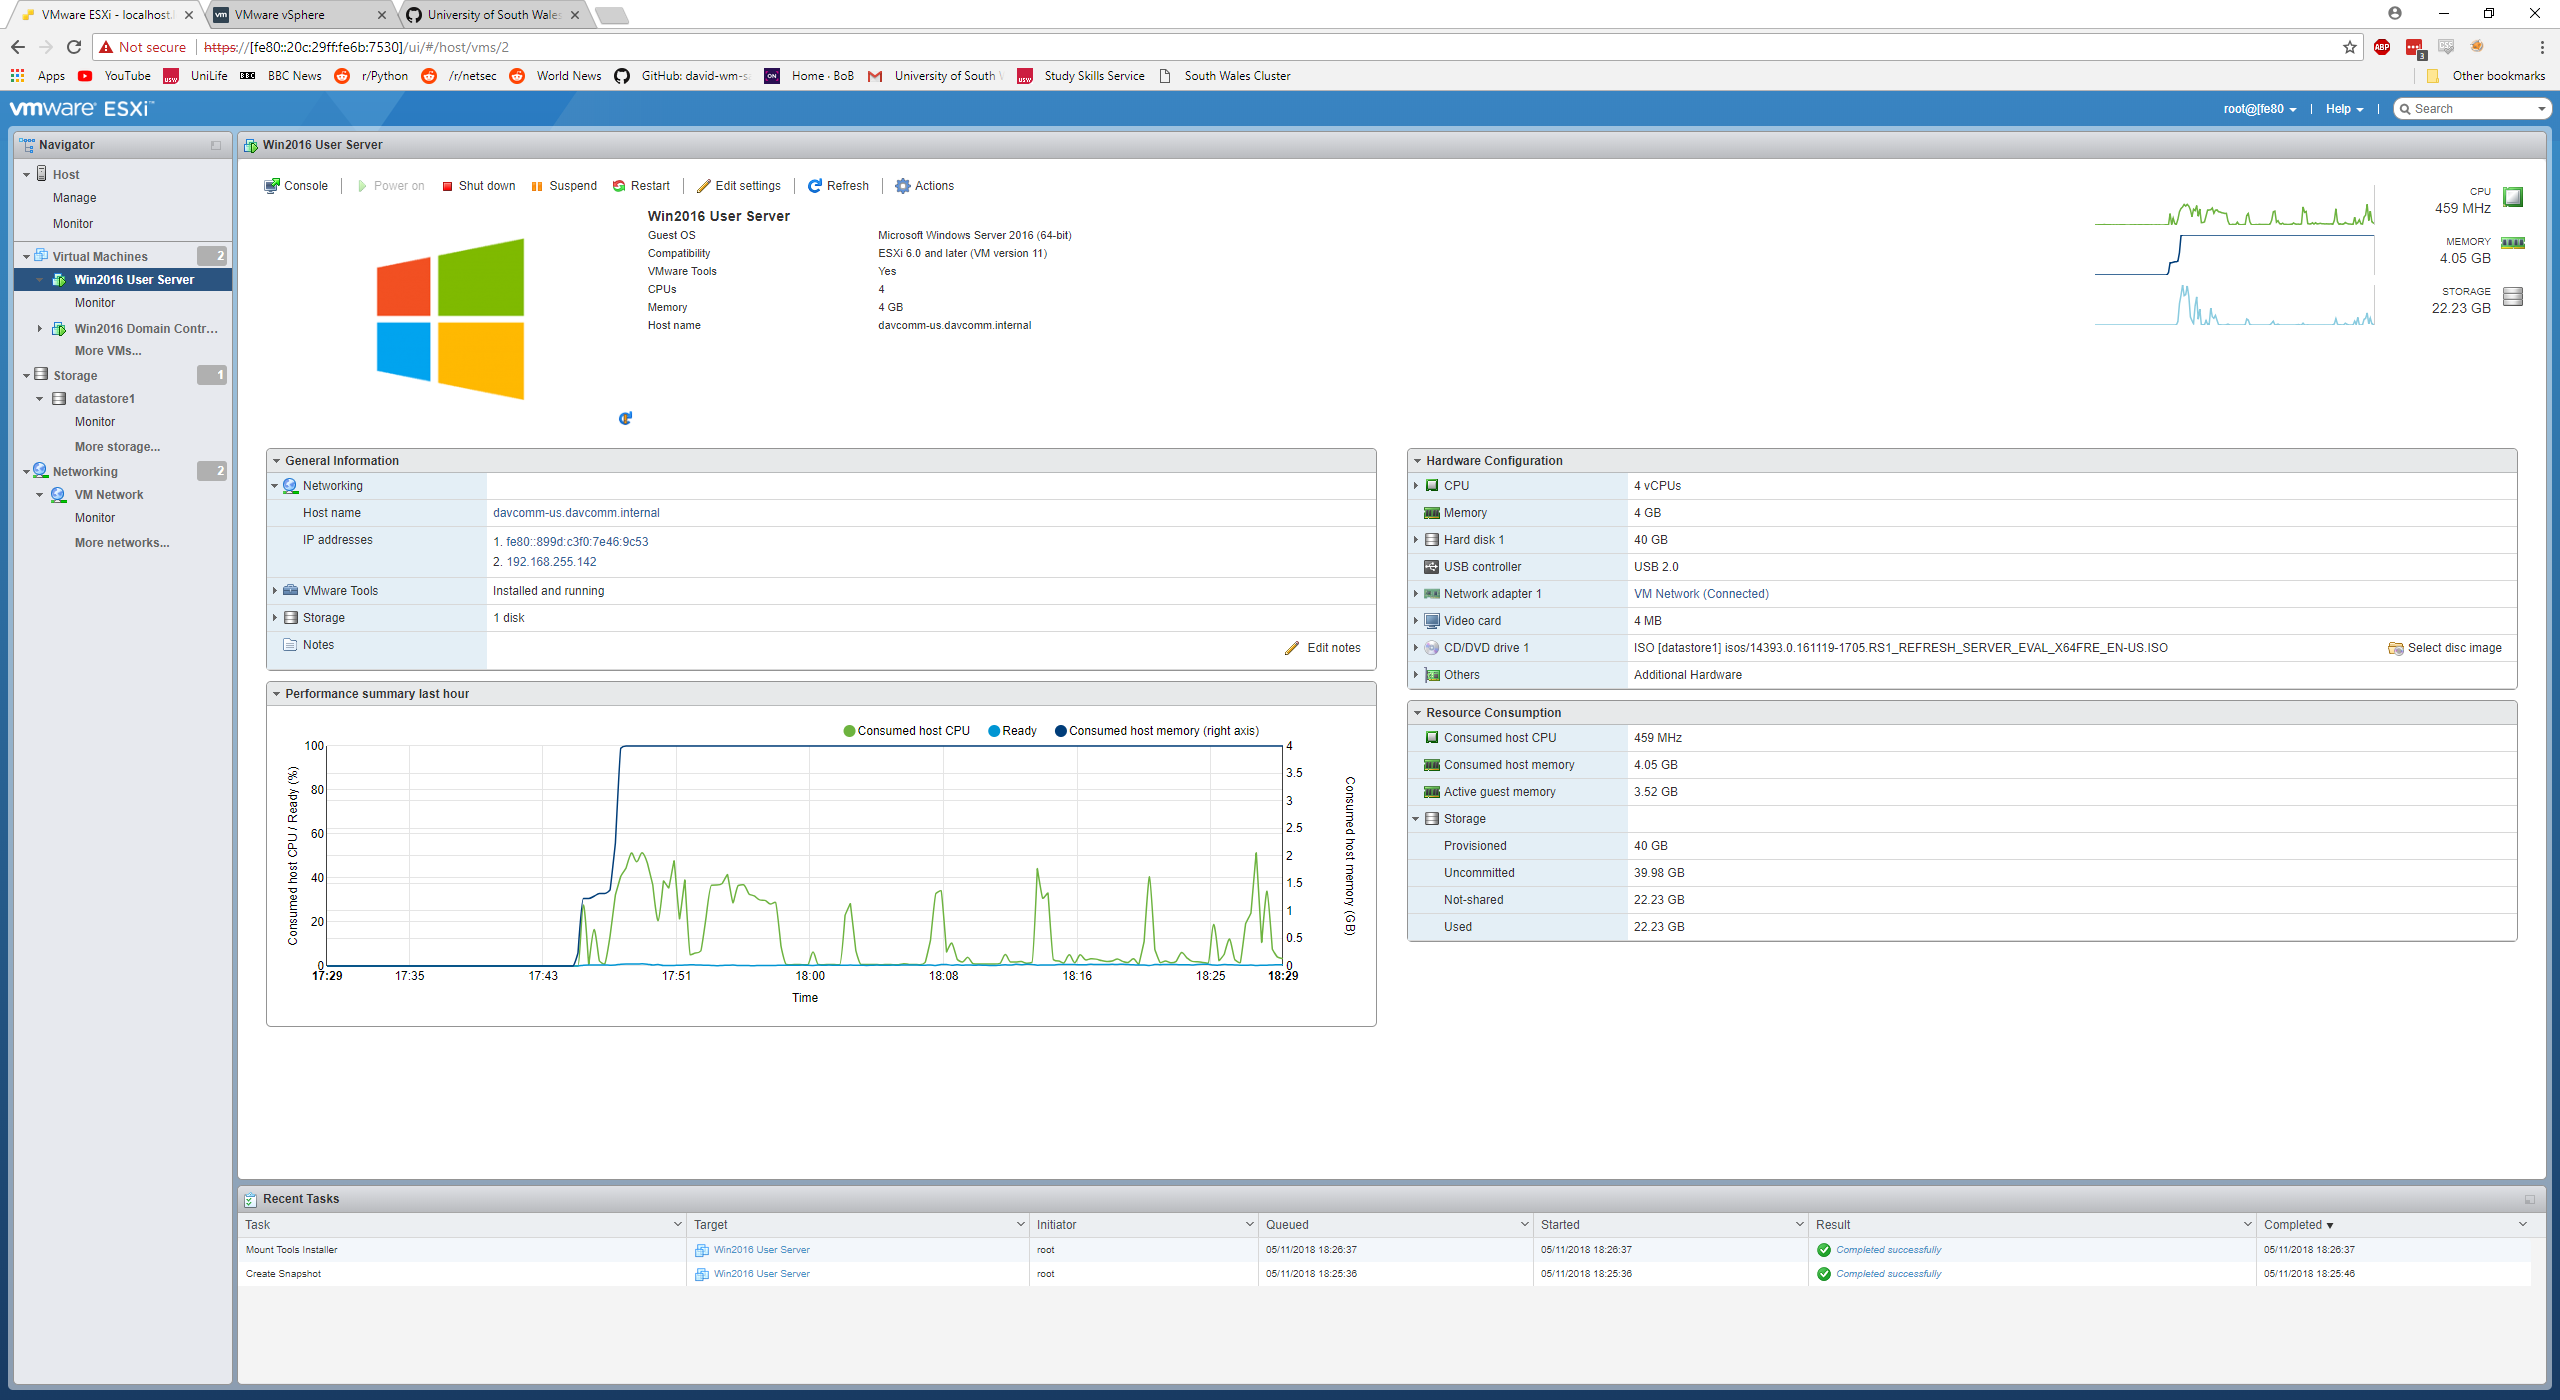
\includegraphics[width=\textwidth]{task2_9_winserver2016us_8}
      \caption{\todo{replace this with a proper figure description}}
      \label{fig:task2:vspherec_us8}
    \end{figure}
  \item \todo{Add file server role}
    \begin{figure}[H]
      \centering
      \captionsetup{skip=2pt}
      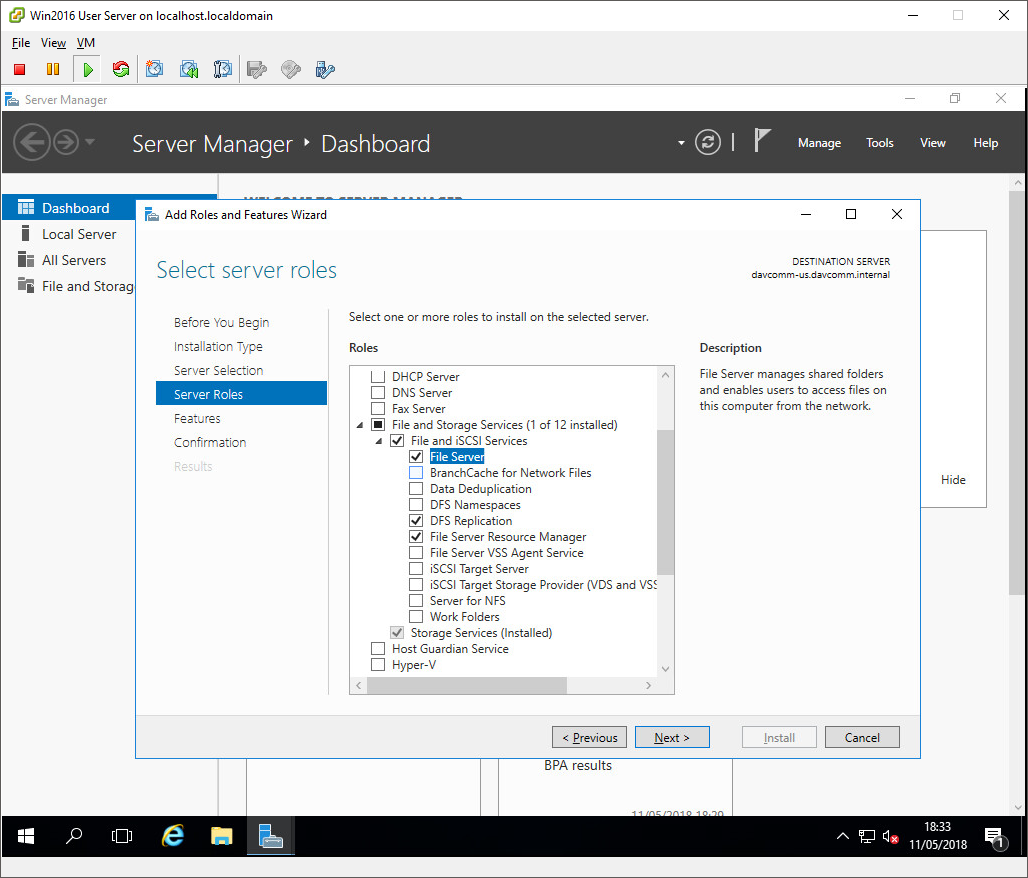
\includegraphics[width=\textwidth]{task2_9_winserver2016us_9}
      \caption{\todo{replace this with a proper figure description}}
      \label{fig:task2:vspherec_us9}
    \end{figure}
  \item \todo{set failover clustering role}
    \begin{figure}[H]
      \centering
      \captionsetup{skip=2pt}
      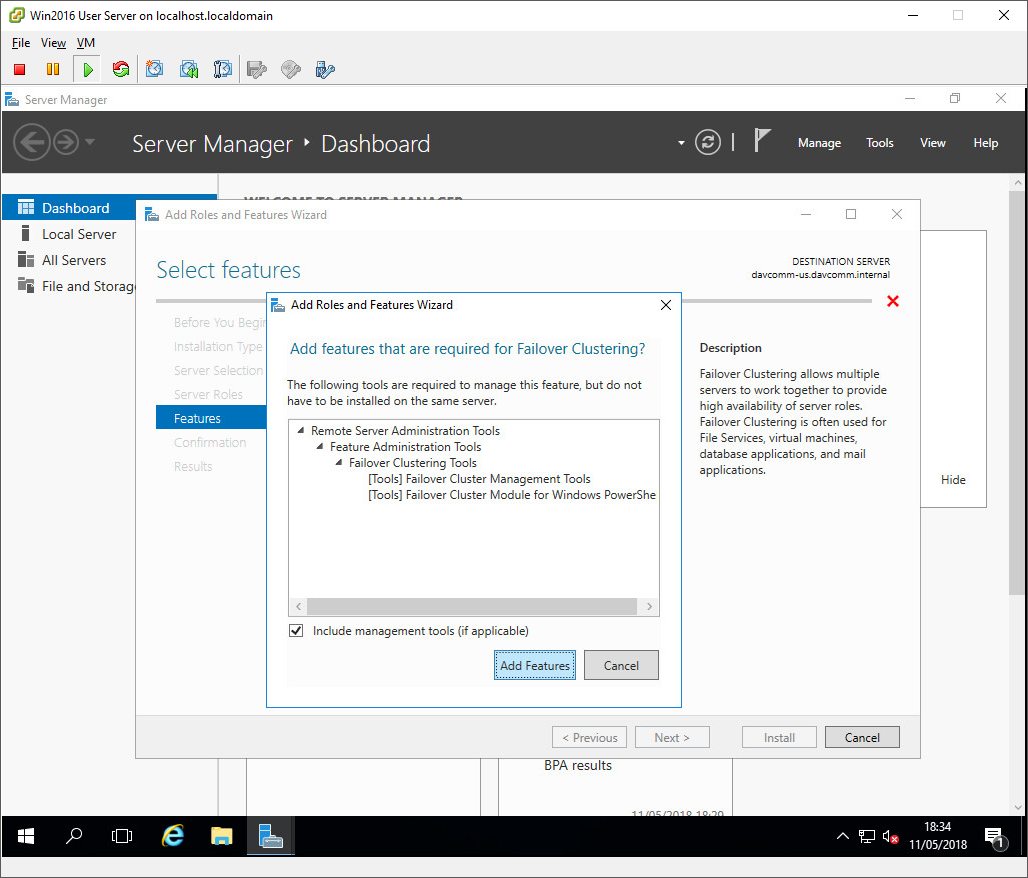
\includegraphics[width=\textwidth]{task2_9_winserver2016us_10}
      \caption{\todo{replace this with a proper figure description}}
      \label{fig:task2:vspherec_us10}
    \end{figure}
  \item \todo{confirm installation selections}
    \begin{figure}[H]
      \centering
      \captionsetup{skip=2pt}
      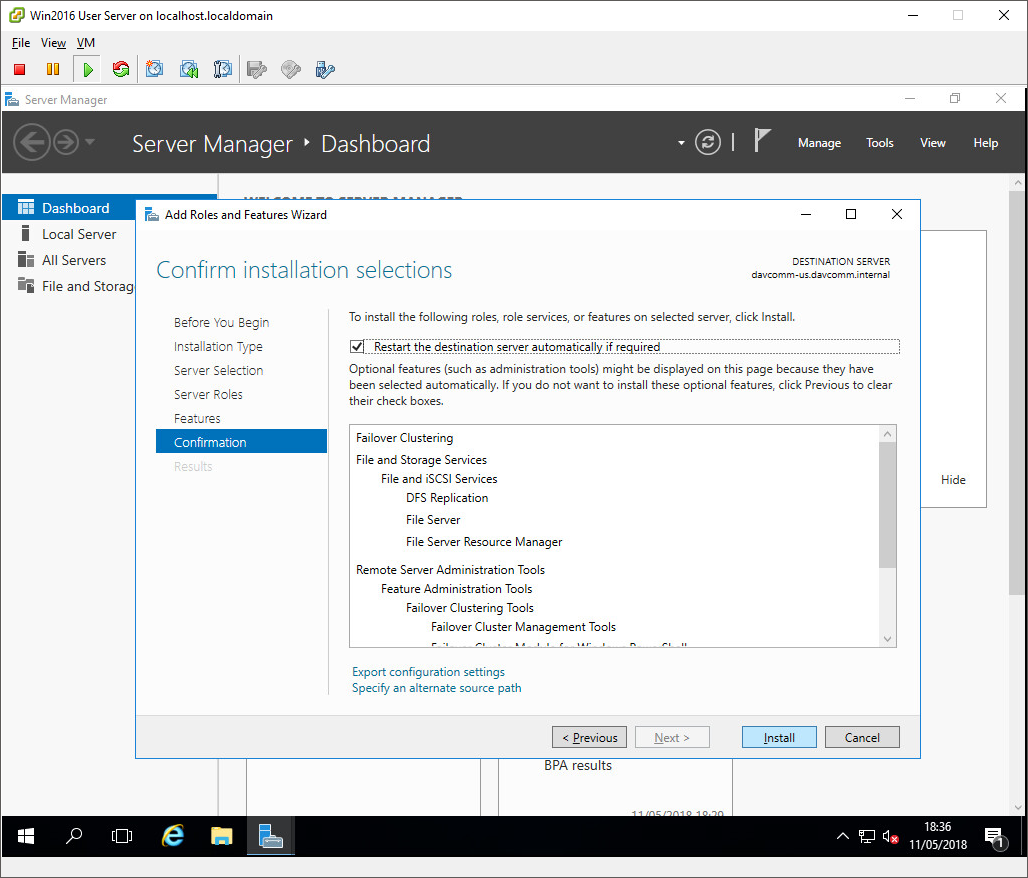
\includegraphics[width=\textwidth]{task2_9_winserver2016us_11}
      \caption{\todo{replace this with a proper figure description}}
      \label{fig:task2:vspherec_us11}
    \end{figure}
\end{enumerate}
\subsubsection{\todo{Set up a user store shared folder}}
\todo{some stuff here...}
\subsubsection{\todo{Create a failover configuration}}
\todo{ahhhhh, how? \url{https://docs.vmware.com/en/VMware-vSphere/6.0/vsphere-esxi-vcenter-server-601-setup-mscs.pdf}}
